\chapter{Aplicação de \emph{Machine Learning} no projeto}
No projeto \emph{TomatoHealth}, que possui a funcionalidade de detecção de doenças em imagens de folhas de tomate, as técnicas de \emph{Machine Learning} desempenham um papel fundamental. No campo da visão computacional aplicada à agricultura, é comum o uso de modelos de Inteligência Artificial para tarefas como classificação de imagens ou detecção de objetos.

Esses métodos tornam-se indispensáveis em situações onde a complexidade do problema torna impraticável ou mesmo impossível desenvolver um programa de computador tradicional baseado em regras fixas capaz de oferecer uma boa solução. Como por exemplo, determinar a doença presente em uma folha a partir de sua imagem. Em casos como esse, recorremos a técnicas de aprendizado de máquina, que oferecem a capacidade de aprender padrões complexos a partir de dados.

No contexto de aprendizado de máquina supervisionado, é necessário dispor de um conjunto de dados rotulados. Esses dados são usados para treinar o modelo de IA, permitindo que ele aprenda a identificar os padrões que caracterizam cada rótulo. Uma vez treinado, o modelo é capaz de generalizar esse conhecimento para realizar predições precisas em novos dados de entrada, predizendo seus rótulos.

\section{Classificação vs Detecção}
Para que o processo de treinamento do modelo de visão computacional seja possível, primeiro é necessário escolher a arquitetura de rede neural que será utilizada. Contudo, ainda antes disso, é necessário definir qual é a tarefa que devemos realizar e um \emph{dataset} já existente para efetuar o treinamento desse primeiro modelo que será integrado à plataforma.

Até agora, a expressão: ``detecção de doenças em imagens de folhas de plantas''; que resume qual é o objetivo do modelo de visão computacional incorporado ao \emph{TomatoHealth} ainda não foi muito bem definida.

É importante esclarecer isso pois, nesse domínio, não há um consenso entre os \emph{datasets} publicamente disponíveis. Isso ocorre pois a tarefa proposta pelo \emph{dataset PlantVillage}, e, portanto, a tarefa mais popular nesse domínio, é a de {\bf classificação}. Isto é, o modelo treinado recebe uma imagem como entrada e então classifica essa imagem como tendo um dentre os diversos rótulos possíveis.

Já o \emph{dataset PlantDoc}, propõe uma tarefa de {\bf detecção de objetos}. Como já comentado, esse \emph{dataset} surgiu para ser uma alternativa ao \emph{PlantVillage}. Podemos comentar sobre a mudança das caracteríticas das imagens, que no \emph{PlantDoc} são oriundas do campo e não obtidas em um ``ambiente controlado'', mas uma das melhorias conceituais mais importantes que foi proposta é justamente a mudança da tarefa de classificação para a de detecção de objetos.

Ao pensar no domínio da agricultura e nos casos de uso dessa tecnologia de visão computacional para identificar doenças em folhas de plantas, não é difícil perceber que a tarefa de detecção de objetos é a mais adequada. 

Para que a tarefa de classificação de imagens seja coerente nesse contexto, é necessário que somente uma folha esteja presente na imagem. Para isso, um agricultor no campo teria de retirar a folha da planta, colocá-la sobre uma supefície plana e então efetuar a captura da imagem.

Já no caso da tarefa de detecção de objetos, bastaria identificar a planta de interesse e efetuar a captura da imagem de modo que as folhas afetadas pela doença estejam presentes na imagem.

Ao compararmos essas duas abordagens diferentes, a etapa adicional inerente à tarefa de classificação (de ser necessário retirar uma folha da planta e só então efetuar a captura da imagem) só seria justificada se isso significasse em uma performance muito superior dos modelos de visão computacional baseadas no conceito de classificação, o que não é o caso \citep{Singh2020}.

Desse modo, é mais interessante trabalharmos com a tarefa de detecção, em que, dado uma imagem de planta com diversas folhas, as folhas presentes na imagem serão detectadas e então classificadas de acordo com as diversas doenças possíveis.

Considerando o fato do \emph{PlantDoc} ter sido construído após a constatação de que haviam problemas profundos com o \emph{PlantVillage} e ter proposto essas melhorias para tentar se consolidar como um novo padrão de \emph{dataset} público para essa tarefa, decidimos escolhê-lo para ser o \emph{dataset} de base para o modelo de visão computacional do \emph{TomatoHealth}.

Para performar essa tarefa de detecção de objetos, escolhemos a família de modelos \emph{YOLO}, que explicaremos em detalhes na seção \ref{sec:modelo}

\section{Entendendo detecção de objetos em \emph{Machine Learning}}
A detecção de objetos tem o objetivo de resolver uma das questões fundamentais de aplicações de visão computacional. Identificar o que são os objetos e onde eles estão localizados nas imagens. Isso é feito por meio da detecção de instâncias de objetos pertencentes a classes específicas nas imagens em questão, com o uso de \emph{bounding boxes} --- retângulos que envolvem os objetos detectados e indicam sua classe \citep{Zou2019Object}.

\begin{figure}[htb!]
    \centering
    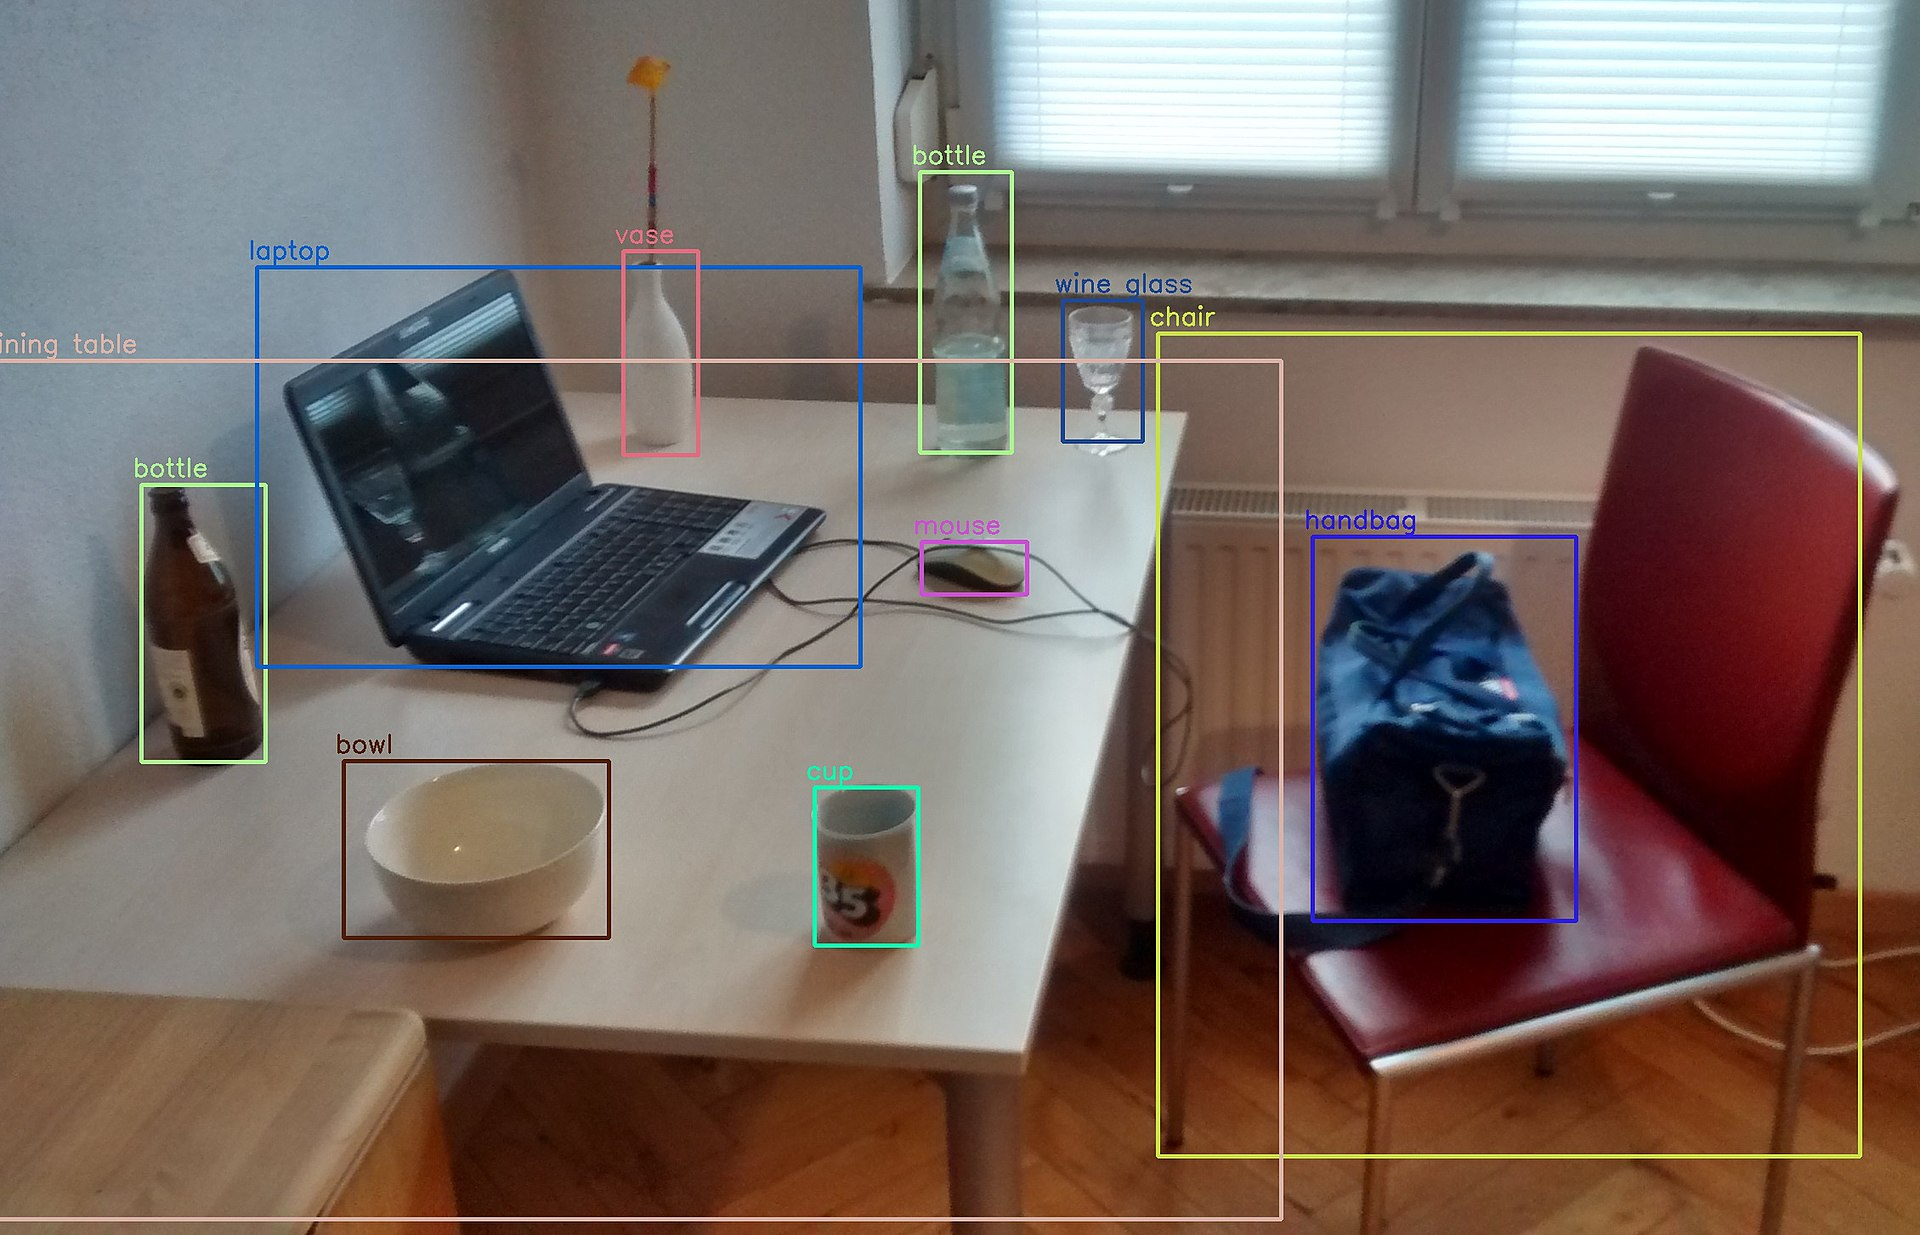
\includegraphics[width=0.8\linewidth]{images/bounding_boxes.png}
    \caption{\label{fig:bounding_boxes} Exemplo de detecção de objetos em uma imagem utilizando bounding boxes. Imagem extraída de \citeauthor{MTheiler}, trabalho próprio, licenciada sob CC BY-SA 4.0. Disponível em: \url{https://commons.wikimedia.org/w/index.php?curid=75843378}.}
\end{figure}

A tarefa de detectar objetos em imagens não é nova, e por ter muitas aplicações como detecção de faces e corpos humanos e servir como base para outras tarefas como direção autônoma, \emph{image captioning} --- que corresponde à tarefa de descrever imagens com textos de linguagem natural ---, aplicações em sistemas com câmeras de segurança, etc. Há uma evolução rápida nesse campo da ciência desde os anos 1990 \citep{Zou2019Object, Zhao2018Object}. Podemos observar essa evolução ao considerarmos o crescimento exponencial no número de publicações que vêm ocorrendo nessa área de conhecimento:
\begin{figure}[htb!]
    \centering
    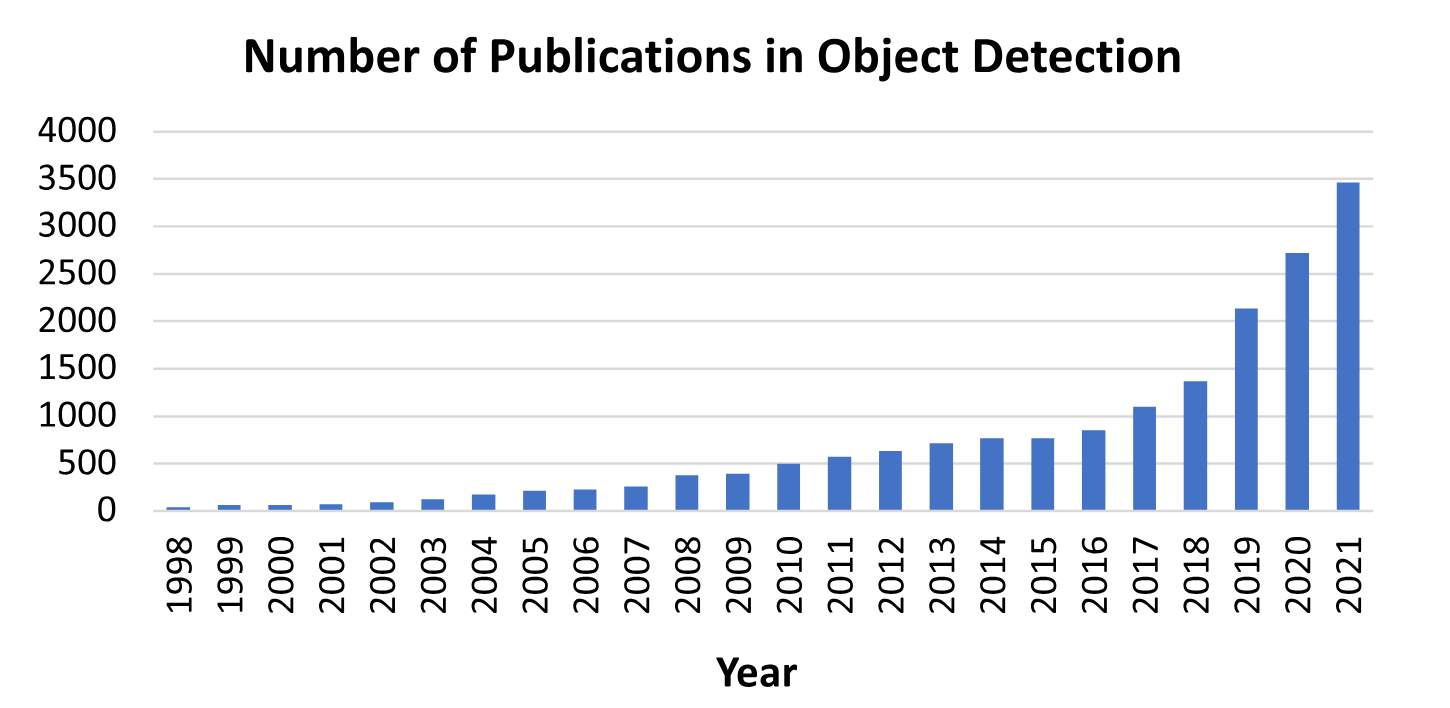
\includegraphics[width=0.8\linewidth]{images/obj_detection_evo.png}
    \caption{\label{fig:obj_evo}Crescimento do número de publicações relacionadas à detecção de objetos ao longo dos anos. (extraído de \citep{Zou2019Object}).}
\end{figure}

O motivo da aceleração significativa na produção de conhecimento científico nessa área do conhecimento foi uma mudança de paradigma considerável: a introdução de técnicas de \emph{deep learning} nessa tarefa de visão computacional. Dessa forma, podemos afirmar que a história da detecção de objetos pode ser compreendida a partir de dois períodos históricos que iremos abordar a seguir: detecção de objetos com uma abordagem tradicional (anterior a 2014) e detecção de objetos baseada em \emph{deep learning} (depois de 2014) \citep{Zou2019Object}.

\subsection{Detecção de objetos com uma abordagem tradicional}
Antes do advento das técnicas de \emph{deep learning}, os métodos para detecção de objetos em imagens dependiam da extração manual de representações (características) eficazes para a inferência esperada. Os algoritmos mais eminentes dessa época utilizavam janelas deslizantes na imagem com filtros compostos pelas características extraídas manualmente. 

Por exemplo, no algorítimo de Viola-Jones, a imagem é percorrida por janelas deslizantes de diversas escalas contendo características presentes em rostos humanos (Haar \emph{features}). Dessa forma, a depender da correspondência das características com a imagem, uma face poderia ser acusada como detectada ou não naquela localidade, isso é feito com classificadores em cascata \citep{Viola}.

Por outro lado, o método \emph{HOG (Histogram of Oriented Gradients)} é um método em que as caraterísticas da imagem são obtidas por meio da computação de gradientes em pequenas porções da imagem. Para cada pequena localidade, o histograma resultante era concatenado aos demais, formando um mapa de características representativo de bordas e texturas. Com a aplicação desse mapa de características em classificadores como \emph{SVMs} (\emph{Support Vector Machines} \citep{Cortes1995Support-Vector}), é possível detectar objetos e essa combinação foi inicialmente implementada para detecção de faces \citep{HOG}.

De maneira geral, perceba que podemos resumir as abordagens tradicionais de detecção de objetos como a extração manual de características das imagens (Haar \emph{features} ou mapas de gradientes oriundos de \emph{HOG}) e então essas características passavam por classificadores simples \citep{Viola, HOG}.

Contudo, essas abordagens eram limitadas e os novos métodos com \emph{deep learning} superaram os desempenhos desses algoritmos mais tradicionais \citep{Zou2019Object}.

\subsection{Detecção de objetos baseada em \emph{deep learning}}
Depois de um tempo, a performance de detectores de objetos com representações extraídas manualmente chegou a ficar saturada. Então, com o advento das técnicas de \emph{deep learning}, especialmente das redes neurais convolucionais (\emph{CNNs}), passou a ser possível processar imagens em seu formato bruto e obter automaticamente representações de alto nível de suas características. Isso impulsionou um avanço significativo na precisão e eficiência dos métodos de detecção de objetos, marcando um salto evolutivo nessa tarefa de visão computacional \citep{Zou2019Object}.

\subsubsection{Fundamentos de redes neurais convolucionais}
Redes neurais podem ser entendidas como funções não lineares extremamente complexas. Esse artifício matemático é constituído por nós --- neurônios --- organizados em camadas. Cada nó efetua uma combinação linear dos valores oriundos dos nós da camada anterior e então passa o resultado dessa operação por uma função não linear --- função de ativação. 

Podemos pensar que a relação entre os dados de entrada de um \emph{dataset} e cada um dos seus rótulos é regida por uma função. Por meio do método do gradiente descendente e da técnica de \emph{backpropagation}, conseguimos fazer com que os parâmetros da rede neural (pesos das combinações lineares) se adaptem de modo a reproduzir essa função.

As redes neurais convolucionais são uma evolução das redes neurais convencionais. Elas são especialmente boas lidando com imagens. São constituídas por três tipos de camadas diferentes:

\paragraph{Camadas convolucionais} aplicam a operação de convolução nos dados que chegam à essa camada. Nesse caso, os pesos do \emph{kernel} da convolução são aprendidos como parâmetros da rede neural.

\paragraph{Camadas de \emph{pooling}} são camadas utilizadas para redimensionar os dados de entrada. Tanto aqui quanto em relação às camadas convolucionais, podemos pensar que os dados de entrada são imagens. Geralmente, as camadas de \emph{pooling} não apresentam parâmetros aprendíveis pela rede (treináveis). A técnica mais utilizada é a denominada \emph{max-pooling}, em que a camada visa preservar o sinal privilegiado pela camada convolucional anterior.

\paragraph{Camadas \emph{fully connected}} são camadas semelhantes às presentes nas redes neurais originais. Geralmente são utilizadas para relacionar --- de maneira treinável --- os resultados das camadas abordadas anteriormente. Constituem camadas que utilizam as características extraídas pelas camadas convolucionais e de \emph{pooling}, para efetuar a classificação. Isso, no caso de um problema de classificação, evidentemente.

\subsubsection{Principais modelos para detecção de objetos com \emph{deep learning}}
Com o avanço do \emph{deep learing} e das redes convolucionais, esses novos conceitos foram introduzidos ao contexto de detecção de objetos com a introdução de \emph{Regions with CNN features} (\emph{RCNNs}) \citep{Zou2019Object, rcnn1, rcnn2}.

A ideia por trás do conceito de \emph{RCNN} é bem direta. Primeiro um conjunto de regiões na imagem é obtido por meio de algoritmos de busca. Depois disso, as representações de cada região é obtida ao passá-las (adaptadas para um tamanho fixo) por uma rede convolucional. Por fim, classificadores como \emph{SVMs} \citep{Zou2019Object}.

Ao longo do tempo, esforços foram sendo feitos para aumentar a velocidade da detecção de objetos com \emph{CNNs}. A abordagem de \cite{SPPNet} utiliza o conceito de \emph{spatial pyramidal pooling}, com esse conceito, as regiões de interesse (\emph{RoI}) são obtidas diretamente no mapa de \emph{features}, o que aumenta muito a velocidade de todo o processo.

O \emph{spatial pyramidal pooling} funciona ao subdividir a \emph{RoI} em ``grades de células'' e aplicar a operação de \emph{max pooling} em cada célula. Desse modo, ao final do \emph{spatial pyramidal pooling}, teremos um vetor de representações de tamanho fixo, independente do tamanho da \emph{RoI} \citep{SPPNet}. Depois disso, esses vetores passam por algoritmos de classificação como \emph{Support Vector Machines (SVMs)}. A possibilidade de uso desse vetor de tamanho fixo foi uma das principais contribuições da \emph{SPPNet} \citep{Zou2019Object}.

Depois disso, \cite{fastRCNN} introduziu a \emph{Fast R-CNN}, que possibilitou o treinamento de uma única rede neural capaz de realizar simultaneamente a regressão das \emph{bounding boxes} (isto é, um ajuste fino das \emph{RoIs} inicialmente propostas por algoritmos de busca) e das classificações. Isso representou um avanço em relação à \emph{SPPnet}, que processava a obtenção das \emph{RoIs} e a classificação das regiões de interesse em etapas distintas, o que tornava o processo mais lento e menos eficiente.

É notável que, a princípio, os métodos de detecção baseados em \emph{CNNs} eram baseados em duas etapas: a proposta das regiões de interesse e, depois, a classificação dessas regiões. A partir de 2015, a tarefa de detecção de objetos com \emph{CNNs} passou a ser feita em somente uma etapa. 

A arquitetura \emph{YOLO (You Only Look Once)} é uma grande representante dessa nova abordagem, permitindo obter as coordenadas das \emph{bounding boxes} e suas classificações em uma única passagem pela rede neural, viabilizando a detecção de objetos em tempo real. Pioneira na detecção de objetos em uma etapa, a arquitetura \emph{YOLO} ganhou popularidade por seus bons resultados em acurácia e velocidade \citep{Zou2019Object}, sendo, por isso, a escolhida para a tarefa de detecção de objetos no \emph{TomatoHealth}.

\section{\emph{YOLO} (\emph{You Only Look Once}) \label{sec:yolo}}
\label{sec:modelo}
\subsection{Contextualização}
A arquitetura de rede neural para detecção de objetos \emph{YOLO} foi introduzida em 2016 com o trabalho de \cite{yolo}. Desde então, diversas evoluções e melhorias foram incorporadas ao modelo. Ao longo dos anos, novas versões dessa arquitetura foram lançadas, indo do \emph{YOLOv1} ao \emph{YOLOv8} em 2023 e até mesmo modelos mais atuais como o \emph{YOLO11}, lançado em 2024 \citep{yolo, yolov8_2023, yolo11_2024}. Por haver mais informação disponível sobre o modelo \emph{YOLOv8} e pelo fato de ainda ser um modelo novo e com performances muito satisfatórias, essa foi a arquitetura escolhida para o projeto. Além disso, apesar dessa evolução entre versões, os conceitos fundamentais e as ideias por trás do \emph{YOLO} ainda podem ser utilizadas para entender seu funcionamento.


Na aplicação \emph{TomatoHealth}, utilizamos o modelo \emph{YOLOv8}. No entanto, o propósito deste texto não é aprofundar em detalhes específicos ou otimizações exclusivas desta versão, mas sim oferecer uma visão geral de como o \emph{framework YOLO} funciona. A seguir, apresentaremos os conceitos primeiro introduzidos em 2016 com o \emph{YOLOv1} e então discutiremos os avanços e melhorias que foram incorporados à arquitetura do \emph{YOLOv8}.

\subsection{Conceitos fundamentais do \emph{YOLO}}
Como já comentado, a principal ideia proposta pela arquitetura \emph{YOLO} é efetuar a detecção de objetos em uma só etapa. Dessa maneira, uma única rede neural faz a predição das \emph{bounding boxes} e das classificações. Com somente um \emph{forward pass}.

\paragraph{Passo a passo do \emph{YOLOv1}:}
No \emph{YOLOv1}, isso é feito por meio do artifício de enxergar o problema de detecção de objetos como puramente um problema de regressão. Isso significa que o problema é formulado de tal modo que os valores preditos pelo modelo são contínuos. Mesmo que a classificação esteja envolvida na tarefa de detecção de objetos, o \emph{YOLOv1} não trabalha com a predição de valores discretos para as classes.

O funcionamento da arquitetura \emph{YOLO} segue o seguinte passo a passo:

\begin{itemize}
    \item Escolhemos uma imagem como \emph{input} para o modelo;
    \item A redimensionamos para um tamanho fixo --- no artigo original, $448 \times 448$;
    \item Dividimos a imagem em $S \times S$ quadrados (\emph{grid cells}) --- no artigo original, $S = 7$;
\end{itemize}

É importante evidenciar que, nesse contexto, cada \emph{grid cell} terá a capacidade de prever um objeto cujo centro esteja localizado no seu interior.

\begin{figure}
    \centering
    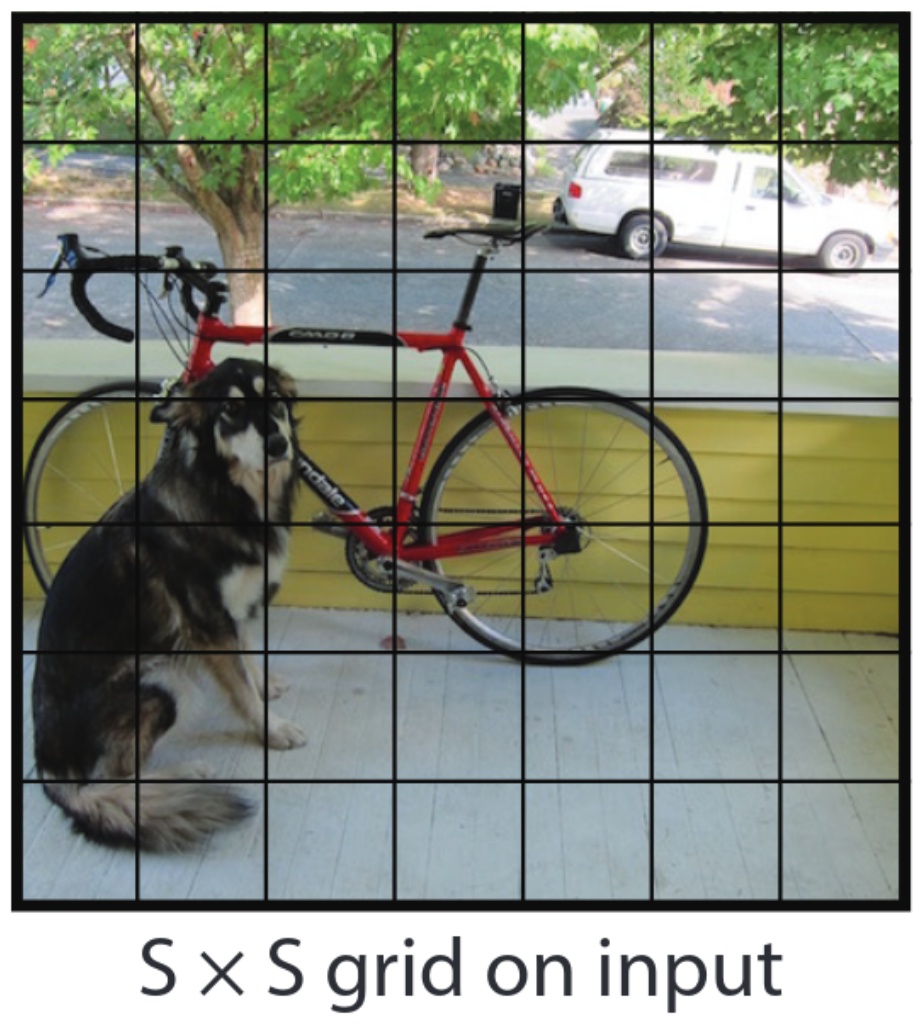
\includegraphics[width=0.5\linewidth]{images/grid_cells.png}
    \caption{\label{fig:grid_cells} Figura que ilustra a as grid cells do YOLOv1 em uma imagem. Imagem extraída de \cite{yolo}.}
\end{figure}

Para treinar o modelo \emph{YOLOv1}, considere o seguinte rótulo de \emph{bounding box}:$(x, y, w, h)$; onde $(x,y)$ corresponde ao centro da \emph{bounding box} e $w$ e $h$ à sua largura e altura, respectivamente. Perceba que no rótulo, os valores de $x, y, w$ e $h$ são valores absolutos relativos aos \emph{pixels} da imagem inteira. Contudo, a previsão do modelo e, portanto, os valores alvo são relativos à \emph{grid cell} em que o centro da \emph{bounding box} está localizado. Dessa forma, uma importante etapa de pre-processamento dos dados que passam pela arquitetura do \emph{YOLOv1} é a normalização desses valores para que sejam relativos à \emph{grid cell}. Isso é feito da seguinte maneira:

Os componentes de uma \emph{bounding box} predita são: $(\Delta{x}, \Delta{y}, \Delta{w}, \Delta{h})$; onde:

\begin{align}
\Delta{x} = \left(x - x_a \right) / \left( L / S\right)\\
\Delta{y} = \left(y - y_a \right) / \left( L / S\right)
\end{align}

Perceba que $\left( L / S\right)$ é justamente o tamanho do lado de uma \emph{grid cell}, pois $L$ é o comprimento do lado da imagem. Além disso, $(x_a, y_a)$ corresponde às coordenadas do canto esquerdo superior da \emph{grid cell}. Desse modo, note que $\Delta{x}$ e $\Delta{y}$ correspondem ao centro da \emph{bounding box} em uma posição relativa à \emph{grid cell} em que ele se encontra.

De maneira análoga:

\begin{align}
\Delta{x} = \left(x - x_a \right) / \left( L / S\right)\\
\Delta{y} = \left(y - y_a \right) / \left( L / S\right)
\end{align}

Então, $\Delta{w}$ e $\Delta{h}$ correspondem ao tamanho da \emph{bounding box} em relação às medidas de uma \emph{grid cell}.

Além desse processamento, outra coisa que deve ser feita é a codificação dos rótulos da classe de cada objeto. Esse processo é chamado \emph{One-hot encoding} e nele, a classe de um objeto é definida por um vetor de tamanho $N$ em que $N$ é a quantidade de classes que o problema possui e é tal que:
\begin{equation}
y_i = 
\begin{cases} 
1, & \text{se } i = k \\
0, & \text{se } i \neq k 
\end{cases}
\end{equation}
onde $i$ representa o índice da classe atual, e $k$ é o índice da classe alvo para o objeto em questão. Ou seja, o vetor resultante do \emph{one-hot encoding} possui valor 1 apenas na posição da classe do objeto e 0 nas demais posições.

Sobre os conceitos envolvidos com as \emph{grid cells} do \emph{YOLOv1}, resta explicar que, cada \emph{grid cell} terá um número $B$ de \emph{bounding boxes} candidatas a englobarem o objeto cujo centro está dentro de seus limites. No artigo original, $B = 2$. Assim, a \emph{bounding box} que tiver o maior valor de confiança de que contém um objeto será a escolhida como \emph{bounding box} para essa \emph{grid cell}.

Para continuar o entendimento dos passos envolvidos na detecção de objetos do \emph{YOLOv1}, precisamos saber como é o resultado da tarefa de detecção de objetos sobre uma imagem. Desse modo, após o \emph{forward pass}, temos o seguinte vetor de predição:

$$
\left[
\Delta\hat{x}_1, \, \Delta\hat{y}_1, \, \Delta \hat{w}_1, \, \Delta\hat{h}_1, \, \hat{c}_1, \, \Delta\hat{x}_2, \, \Delta\hat{y}_2, \, \Delta\hat{w}_2, \, \Delta \hat{h}_2, \, \hat{c}_2, \, \hat{p}_1, \, \hat{p}_2, \, \dots, \, \hat{p}_{20} 
\right]
$$

onde:
$$
\left[
\Delta\hat{x}_i, \, \Delta\hat{y}_i, \, \Delta \hat{w}_i, \, \Delta\hat{h}_i, \, \hat{c}_i
\right]^B_{i=1}
$$

Corresponde às coordenadas das \emph{bounding boxes} preditas pela \emph{grid cell} em questão e $\hat{c}$ a confiança de que, nessa \emph{grid cell} o centro de um objeto esteja localizado.

Além disso, 

$$
\left[
\hat{p}_1, \, \hat{p}_2, \, \dots, \, \hat{p}_{20} 
\right]
$$

São os valores das probabilidades preditas para cada classe, no modelo proposto por \emph{One-hot encoding}. Temos o número de 20 classes pois o \emph{YOLOv1} foi concebido para atuar com o \emph{dataset} PASCAL VOC \citep{yolo}.

Assim, para cada \emph{grid} cell, temos um vetor de tamanho $1 \times 30$ de resultado. Como são $7 \times 7$ \emph{grid cells} em uma imagem, temos de resultado de um \emph{forward pass} um vetor de tamanho $7 \times 7 \times 30$.

Nesse ponto, perceba que, para obtermos as coordenadas e as dimensões das \emph{bounding boxes}, precisamos passar pelo seguinte processo (estamos revertendo a normalização feita no inicio do \emph{forwar pass}):

$$
\begin{cases}
x_1 = \Delta x_1 \times \left(L / S \right) + x_a \\
y_1 = \Delta y_1 \times \left(L / S \right) + y_a \\
w_1 = \Delta w_1 \times L \\
h_1 = \Delta h_1 \times L
\end{cases}
$$

E, para obter as informações sobre a classe, temos:

\begin{itemize}
    \item \textbf{Classe do objeto}: A classe \( l \) do objeto é dada por:
   $$
   l = \arg\max(p_1, p_2, \dots, p_{20})
   $$

    \item \textbf{Confiança da classe}: A confiança da classe (\( \hat{c}_1 \) ou \( \hat{c}_2 \)) é calculada multiplicando a confiança da \emph{bounding box} pelo valor máximo de probabilidade \( p \) entre as classes. Dessa forma:
       $$
       p = \max(p_1, p_2, \dots, p_{20})
       $$
       e
       $$
       \hat{c} = c_i \times p
       $$
       onde $c_i = \max\{c_1, c_2\}$.
\end{itemize}
Então, ao exibir as informações sobre o objeto detectado, levamos em consideração a confiança $\hat{c}$ e a classe $l$. 

\paragraph{Arquitetura:} A arquitetura do \emph{YOLOv1} é composta basicamente por uma rede neural convolucional convencional. É uma arquitetura inspirada pela \emph{GoogleNet}, em que temos 24 camadas convolucionais e 2 camadas \emph{fully connected} ao final da rede para que possamos obter o vetor de saída desejado. As 24 camadas convolucionais são responsáveis por gerar o mapa de representações da imagem e geralmente constituem uma porção da rede que é chamada de \emph{backbone}. Por outro lado, as camadas \emph{fully connected} são responsáveis por usar o mapa de representações para obter as predições do modelo.

\paragraph{Treinamento do \emph{YOLOv1}}
O treinamento do modelo \emph{YOLOv1} geralmente começa com uma rede neural pré-treinada no \emph{dataset ImageNet} \citep{imagenet}. Depois disso, finalizamos o treinamento (\emph{fine tune}) no \emph{dataset} de detecção de objetos. O processo de treinamento do \emph{YOLOv1} com \emph{dataset} de detecção de objetos pode ser resumido na figura \ref{fig:yolo_train}.

\begin{figure}[htb!]
    \centering
    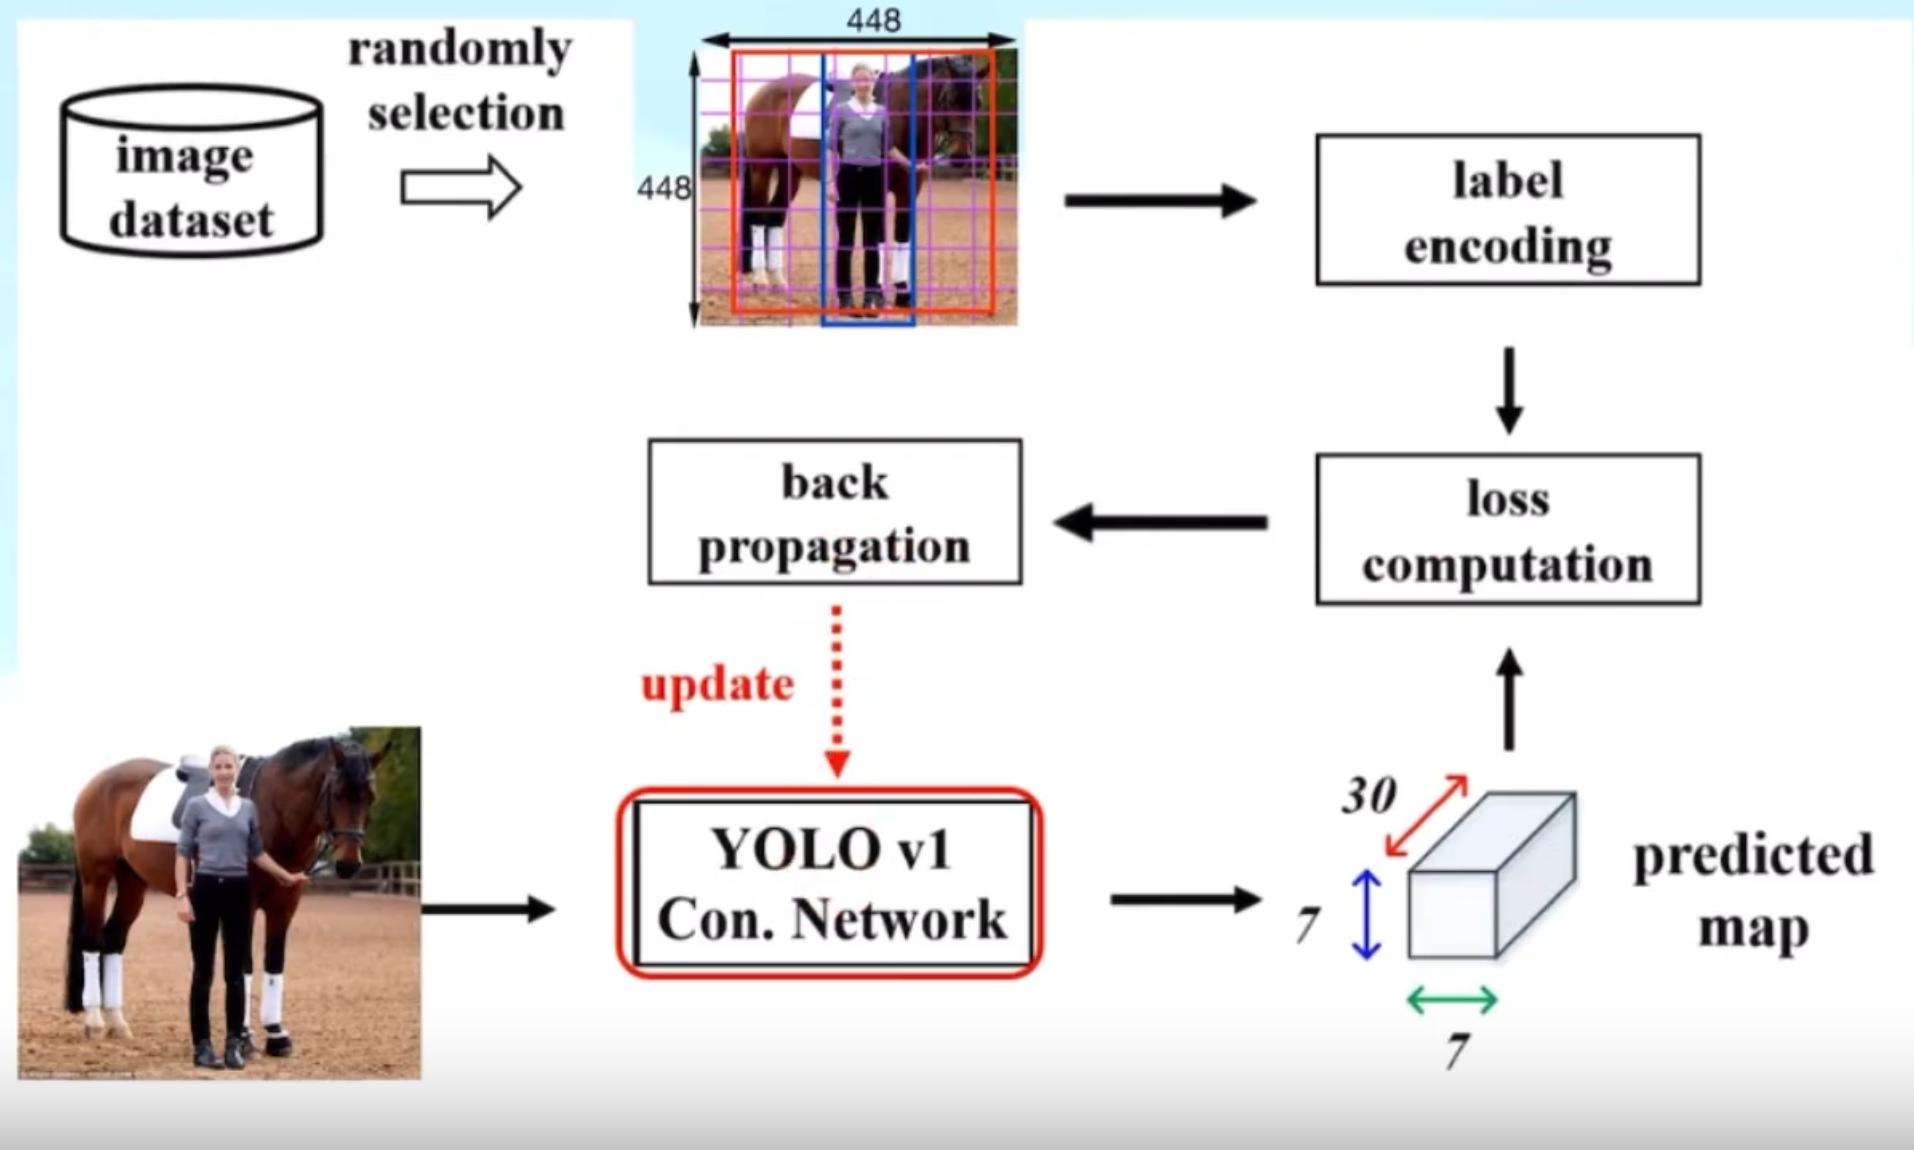
\includegraphics[width=0.8\linewidth]{images/yolo_train.png}
    \caption{\label{fig:yolo_train} Ilustração do processo de treinamento do YOLOv1. Disponível em: \url{https://www.youtube.com/watch?v=zgbPj4lSc58&list=PL1u-h-YIOL0sZJsku-vq7cUGbqDEeDK0a&index=1&t=1517s}.}
\end{figure}

Escolhemos uma imagem aleatória do conjunto de dados, efetuamos o pré-processamento de seus rótulos como comentado, passamos a imagem pela rede neural, computamos a função de perda ao comparar os resultados do \emph{forward pass} com os rótulos processados e então efetuamos o processo de \emph{back propagation}, atualizando os pesos do modelo com base no gradiente da função de perda. 

\paragraph{Função de perda}
A função de perda introduzida pelo \emph{YOLOv1} é a soma das funções de perda por todas as \emph{grid cells}:
\begin{center}
\[
L = \sum_{i=1}^{S^2} L_i
\]
\end{center}
A função de perda é dividida nos casos em que o centro de um objeto está ou não localizado dentro de uma \emph{grid cell}. Isso é feito por meio das funções indicadoras $\mathds{1}_i^{\text{obj}}$ e $\mathds{1}_i^{\text{no\_obj}}$, que assumem respectivamente o valor 1 quando há e não há objetos na \emph{grid cell} $i$, e assumem 0 caso contrário. Além disso, desejamos dar mais importância para a presença de objetos na imagem, por isso, há a constante $\lambda_{\text{no\_obj}}$, que no artigo original tem o valor de 0,5:
\begin{center}
\[
L = \sum_{i=1}^{S^2} \mathds{1}_i^{\text{obj}} \cdot L_{i, \text{obj}} + \lambda_{\text{no\_obj}} \sum_{i=1}^{S^2} \mathds{1}_i^{\text{no\_obj}} \cdot L_{i, \text{no\_obj}}
\]
\end{center}

Agora, vamos definir $L_{i, \text{obj}}$. Essa função é definida como uma soma ponderada da função de perda da confiança de que há um objeto cujo centro está na \emph{grid cell} $i$ (\emph{objectness loss}), a função de perda da classificação e a função de perda das coordenadas da \emph{bounding box}.
\begin{center}
\[
L_{i, \text{obj}} = \lambda_{\text{coord}} \cdot L_{i, \text{obj}}^{\text{box}} + L_{i, \text{obj}}^{\text{conf}} + L_{i, \text{obj}}^{\text{cls}}
\]
\end{center}

No artigo original, $\lambda_{\text{coord}}$ tem o valor de 5.

A função de perda para as \emph{bounding boxes}, \( L_{i, \text{obj}}^{\text{box}} \), é definida como a soma dos erros quadráticos entre os valores preditos e os valores presentes no rótulo da imagem em questão (\emph{ground truth}). A expressão é dada por:

\[
L_{i, \text{obj}}^{\text{box}} = (\Delta x_i - \Delta \hat{x}_i)^2 + (\Delta y_i - \Delta \hat{y}_i)^2 + \left(\sqrt{\Delta w_i} - \sqrt{\Delta \hat{w}_i}\right)^2 + \left(\sqrt{\Delta h_i} - \sqrt{\Delta \hat{h}_i}\right)^2
\]

onde: \( \Delta x_i \) e \( \Delta y_i \) são as coordenadas reais do centro da \emph{bounding box};  \( \Delta \hat{x}_i \) e \( \Delta \hat{y}_i \) são as coordenadas preditas; \( \Delta w_i \) e \( \Delta h_i \) são a largura e a altura reais da \emph{bounding box}; e \( \Delta \hat{w}_i \) e \( \Delta \hat{h}_i \) são os valores preditos.

A raiz quadrada em \( w \) e \( h \) está presente na computação dessa função de perda pois, quanto maior a \emph{bounding box}, maiores serão as diferenças $\left(\Delta w_i - \Delta \hat{w}_i \right)$ e $ \left( \Delta h_i - \Delta \hat{h}_i \right)$. Esse aumento ocorre ainda mais ao usarmos o quadrado dessas diferenças. Por isso, a função de perda penaliza mais caixas maiores. Para tentar melhorar essa situação, a ideia é introduzir a raiz quadrada para diminuir a penalização de caixas de maior tamanho, já que maiores valores em $\left(\Delta w_i - \Delta \hat{w}_i \right)$ e $ \left( \Delta h_i - \Delta \hat{h}_i \right)$, após o uso da raiz quadrada, não impactarão tanto no valor final da função de perda.

Já a função de perda da confiança da presença de centro de objeto na \emph{grid cell} $i$, é somente o erro quadrático da confiança predita e do valor rótulo (nesse caso, sempre $1$).

\begin{center}
\[
L_{i, \text{obj}}^{\text{conf}} =  (c_i - \hat{c}_i)^2
\]
\end{center}

Por fim, a função de perda de classificação também é constituída por erro quadrático.

\begin{center}
\[
L_{i, \text{obj}}^{\text{cls}} = \sum_{c=1}^{20} (p_{i,c} - \hat{p}_{i,c})^2
\]
\end{center}

Em que $p$ e $\hat{p}$ são os vetores das probabilidades.

Agora, precisamos computar a função de perda no caso em que não há objetos cujo centro está localizado na \emph{grid cell} $i$. Nesse caso, somente levamos em consideração a \emph{objectness score}:

\begin{center}
\[
L_{i, \text{no\_obj}} = \sum_{j=1}^{B} (c_{i,j} - \hat{c}_{i,j})^2
\]
\end{center}

Em que o valor de $\hat{c}_{i,j}$ é 0 e $B$ igual a 2.

\paragraph{Limitações}
Apesar de ser uma arquitetura disruptiva que revolucionou o cenário da visão computacional e detecção de objetos, o \emph{YOLOv1} apresentava algumas limitações. Principalmente a incapacidade de detectar muitos objetos, principalmente quando os objetos são pequenos e estão amontoados. (limitação devido às \emph{grid cells}). Além disso, como todas as \emph{bounding boxes} têm sua origem em um processo adaptativo relativo às \emph{grid cells}, o \emph{YOLOv1} tem dificuldade em adaptar as caixas a objetos com proporções variadas \citep{yolo_review}.

\subsection{Métricas}
Para avaliar diferentes modelos de detecção de objetos, temos diversas métricas para quantificar a qualidade do modelo em identificar corretamente objetos em uma imagem. Vamos detalhar as métricas mais comuns, com base nas definições matemáticas do artigo \citep{Padilla2020A}.

\begin{itemize}
    \item {\bf \emph{Intersection over Union (IoU}:} 
    \emph{Intersection over Union} mede a área de sobreposição entre a \emph{bounding box} predita ($B_p$) e a \emph{bounding box} real (\emph{ground truth}) ($B_{gt}$).
    \begin{center}
        \[
        \text{IoU} = \dfrac{\text{Área}\left( B_p \cap B_{gt} \right)}{\text{Área}\left( B_p \cap B_{gt}\right)}
        \]
    \end{center}
    Uma das funções mais importantes dessa métrica é definir:
    \begin{itemize}
        \item Verdadeiros positivos (\emph{TP}): uma detecção correta de uma \emph{bounding box} real (\emph{ground-truth} \citep{Padilla2020A};
        \item Falsos positivos (\emph{FP}): uma detecção incorreta de um objeto inexistente ou uma detecção mal posicionada de um objeto existente \citep{Padilla2020A};
        \item Falsos negativos (\emph{FN}): uma \emph{bounding box} real (\emph{ground-truth}) não detectada \citep{Padilla2020A}.
    \end{itemize}

    Desse modo, consideramos a detecção correta de uma \emph{bounding box} caso a classe detectada seja a correta e $\emph{IoU} > t$.
    \item {\bf Precisão e \emph{Recall}:}
    A \emph{Precisão} (\(P\)) mede a proporção de predições corretas entre todas as predições feitas:
    \[
    P = \frac{\text{TP}}{\text{TP} + \text{FP}}
    \]

    O \emph{Recall} (\(R\)) mede a proporção de objetos reais detectados entre todos os objetos presentes na imagem:
    \[
    R = \frac{\text{TP}}{\text{TP} + \text{FN}}
    \]
    \item {\bf \emph{Average Precision (AP)}:}
    A \emph{Average Precision} (AP) é uma medida que combina a precisão e o \emph{recall}, calculando a área sob a curva de precisão-\emph{recall}. Primeiramente, precisamos entender como obtemos diversos valores de precisão e \emph{recall} para que seja possível traçar essa curva.
    
    Isso é feito ao escolhermos diversos valores $t$ do \emph{threshold} de confiança para classificação. Para cada valor de $t$, obtemos um par de valores de precisão e \emph{recall}. Depois disso, traçamos a curva. Então, um método comum para o cálculo do AP é a \textbf{interpolação em todos os pontos} \citep{Padilla2020A}:
    \[
    AP_{\text{all}} = \sum_{n} (R_{n+1} - R_n) P_{\text{interp}}(R_{n+1})
    \]
    onde onde
    \[
    P_{\text{interp}}(R_{n+1}) = \max_{\tilde{R} : \tilde{R} \geq R_{n+1}} P(\tilde{R}).
    \]
    Uma noção visual pode ser vista na figura \ref{fig:average_precision_curve}.
    \begin{figure}[htb!]
        \centering
        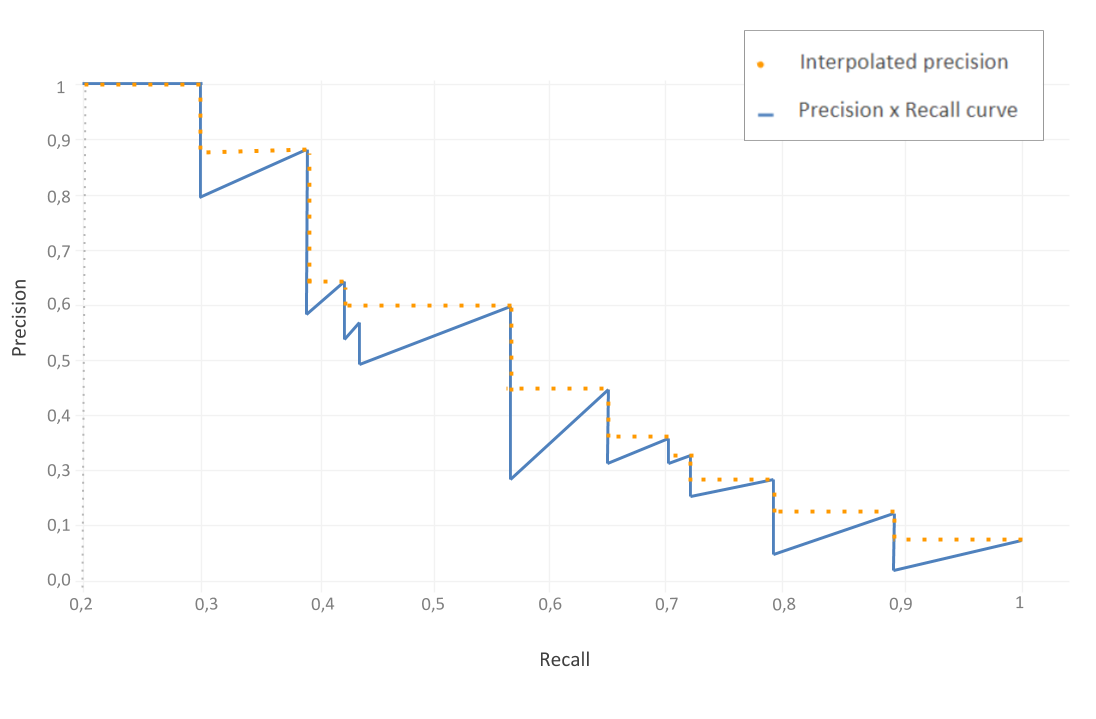
\includegraphics[width=0.8\linewidth]{images/ap.png}
        \caption{\label{fig:average_precision_curve} Exemplo de curva de precisão-recall usando interpolação em todos os pontos para o cálculo da Average Precision (AP). Disponível em: \url{https://manalelaidouni.github.io/assets/img/pexels/all_point_interpolated_AP_(2)-848db820-1379-456f-bad8-8e45ea562fd0.png}.}
    \end{figure}
    
    \item {\bf \emph{Mean Average Precision (mAP)}:}
    A \emph{Mean Average Precision} (mAP) é a média do AP calculada sobre todas as classes em um conjunto de dados. Se um modelo é avaliado em \(N\) classes, a mAP é dada por:

    \[
    mAP = \frac{1}{N} \sum_{i=1}^{N} AP_i
    \]

    Onde \( AP_i \) é a AP para a classe \(i\).

\end{itemize}
Essas métricas, especialmente o AP e o mAP, são amplamente utilizadas para avaliar e comparar o desempenho de diferentes modelos de detecção de objetos. Além disso, há diferentes variantes do mAP para diferentes valores de IoU. Por exemplo, AP@50 (que gera a curva AP com o valor de $t$ em 0,5); AP@75 e AP@50:5:95, que entrega diversos valores.

\subsection{Avanços da família \emph{YOLO}}
\paragraph{\emph{Backbone}, \emph{neck} e \emph{head}:}
Com o avanço das arquiteturas para detecção de objetos, nomenclaturas para diferentes partes das redes neural convolucionais começaram a ser 
utilizadas. Nesse contexto, se destacam o {\bf backbone}, {\bf neck} e {\bf head}. Por isso, como parte da explicação sobre a evolução da família \emph{YOLO}, é interessante abordar a função de cada uma dessas partes dos detectores de objetos.

\begin{figure}[htb!]
    \centering
    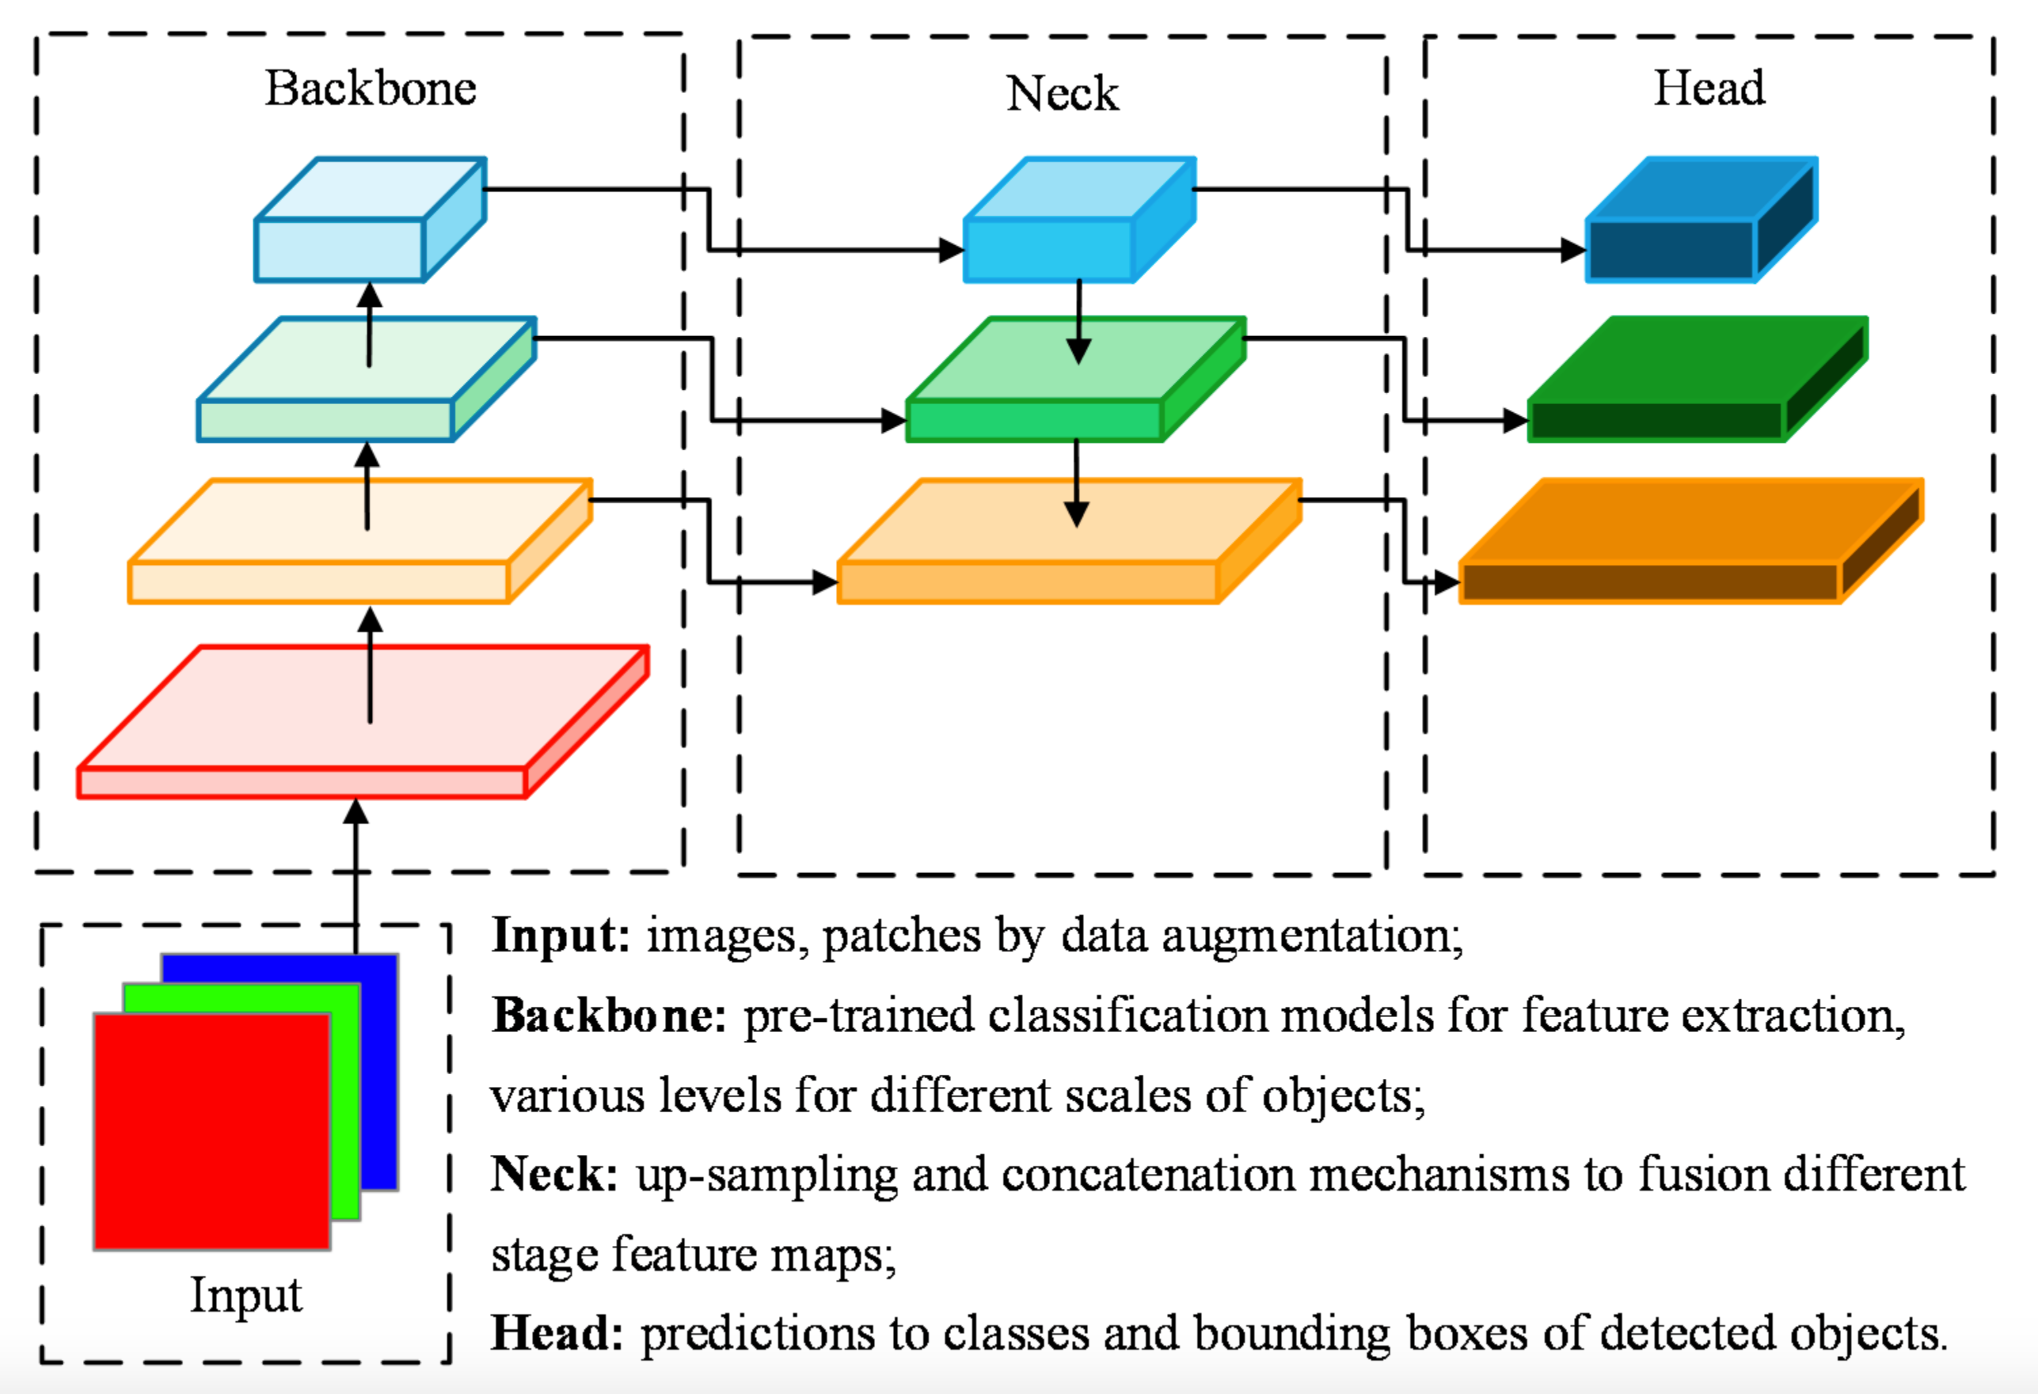
\includegraphics[width=0.8\linewidth]{images/backbone-neck-head.png}
    \caption{\label{fig:backbone_neck_head} Estrutura de detecção de objetos mostrando a separação entre Backbone, Neck e Head. Disponível em: \url{https://velog.io/@peterkim/Object-Detection에서-말하는-Backbone-Neck-Head}.}
\end{figure}

\begin{itemize}
    \item {\bf Backbone:} o \emph{backbone} da rede convolucional, muitas vezes referido como uma rede em si, é muito comum em arquiteturas de modelos de detecção de objetos. A função do \emph{backbone} é realizar a extração das representações da imagem. Além disso, essas características extraídas são codificadas em uma dimensão adequada para o \emph{neck}, que será explicado a seguir. O \emph{backbone} deve ser capaz de capturar representações de alto nível e baixo nível da imagem de entrada \citep{shroff2021know}.
    
    \item {\bf Neck:} depois do \emph{backbone}, o \emph{neck} é responsável por transformar ainda mais as representações que foram extraídas anteriormente. O seu objetivo é melhorar a qualidade dessas representações de modo que elas sejam capazes de fornecer ainda mais informação para a detecção de objetos \citep{shroff2021know}.

    \item {\bf Head:} a \emph{head} do modelo de detecção de objetos é a sua parte final. Ela é responsável por produzir as predições do modelo e se baseia nas informações extraídas pelo \emph{backbone} e \emph{neck} \citep{shroff2021know}.
\end{itemize}

\paragraph{Abordagem baseada em âncoras:}
Desde o lançamento do \emph{YOLOv1}, a abordagem para detecção de objetos evoluiu significativamente. As versões subsequentes introduziram conceitos importantes, como o uso de \emph{âncoras} (\emph{anchors}) no \emph{YOLOv2} e \emph{YOLOv3}. As âncoras são \emph{bounding boxes} predefinidas que servem como referências para o modelo detectar objetos de diferentes escalas e proporções. Isso é feito geralmente utilizando o algoritmo de clusterização não supervisionado \emph{K-means} nas \emph{bounding boxes} presentes nos dados de treinamento do modelo de detecção. Essa técnica melhorou a precisão na detecção, mas adicionou complexidade ao processo \citep{yolo_review}.

\paragraph{\emph{YOLOX}:}
Com o surgimento do \emph{YOLOX} \cite{yolox2021}, foi adotada uma abordagem \emph{anchor-free}, eliminando a necessidade de âncoras predefinidas. Em vez disso, o modelo efetua a regressão das \emph{bounding boxes} diretamente pela \emph{CNN}, simplificando o processo de detecção. Além disso, o \emph{YOLOX} introduziu à família de modelos \emph{YOLO} a abordagem de uma \emph{head} desacoplada, ou seja: cada ``parte'' (\emph{branch}) da \emph{CNN} poderia se especializar na sua tarefa (uma delas na regressão das \emph{bounding boxes} e a outra na tarefa de classificação). Nesse ponto, a tarefa de detecção de objetos na arquitetura \emph{YOLO} deixou de ser uma tarefa centrada em regressão e passou a ser uma tarefa desacoplada de classificação e regressão \citep{yolox2021}. De qualquer forma, é interessante ressaltar que, apesar do desacoplamento, o treinamento é feito de maneira única. Com uma só passagem da imagem pela rede neural, obtemos todos os resultados da tarefa de detecção de objetos, o que não retorna à abordagem tradicional (de detecção em múltiplas etapas).

\paragraph{\emph{YOLOv8:}}
O \emph{YOLOv8}, desenvolvido pela \emph{Ultralytics} e lançado em janeiro de 2023 \citep{yolov8_2023}, incorporou essa abordagem \emph{anchor-free} e introduziu diversas melhorias na arquitetura:

\begin{itemize} 
    \item \textbf{Melhorias no \emph{backbone} e \emph{neck}}: O \emph{YOLOv8} utiliza um \emph{backbone} mais eficiente para extração de representações, aliado a um \emph{neck} aprimorado que facilita a fusão de informações de múltiplas escalas. Isso melhora a capacidade do modelo em detectar objetos de diferentes tamanhos, especialmente objetos pequenos em imagens de alta resolução;

    \item \textbf{Desacoplamento da \emph{head}}: De modo semelhante ao \emph{YOLOX}, o \emph{YOLOv8} implementa uma \emph{head} desacoplada, onde as tarefas de regressão das \emph{bounding boxes} e de classificação são realizadas de forma separada. Essa separação permite otimizar cada tarefa individualmente, aumentando a precisão geral do modelo.

    \item \textbf{Funções de perda específicas}: No processo de treinamento, o modelo utiliza uma combinação de \emph{Complete Intersection over Union} (CIoU) \citep{Zheng2020} e \emph{Distribution Focal Loss} (DFL) \citep{Li2020} na função de perda da regressão das \emph{bounding boxes}. Para a perda de classificação, é empregada a \emph{Binary Cross-Entropy} (BCE). Essa abordagem especializada para cada tipo de perda contribui para melhorias significativas na precisão da detecção \citep{yolo_review}.
\end{itemize}
\begin{figure}[htb!]
    \centering
    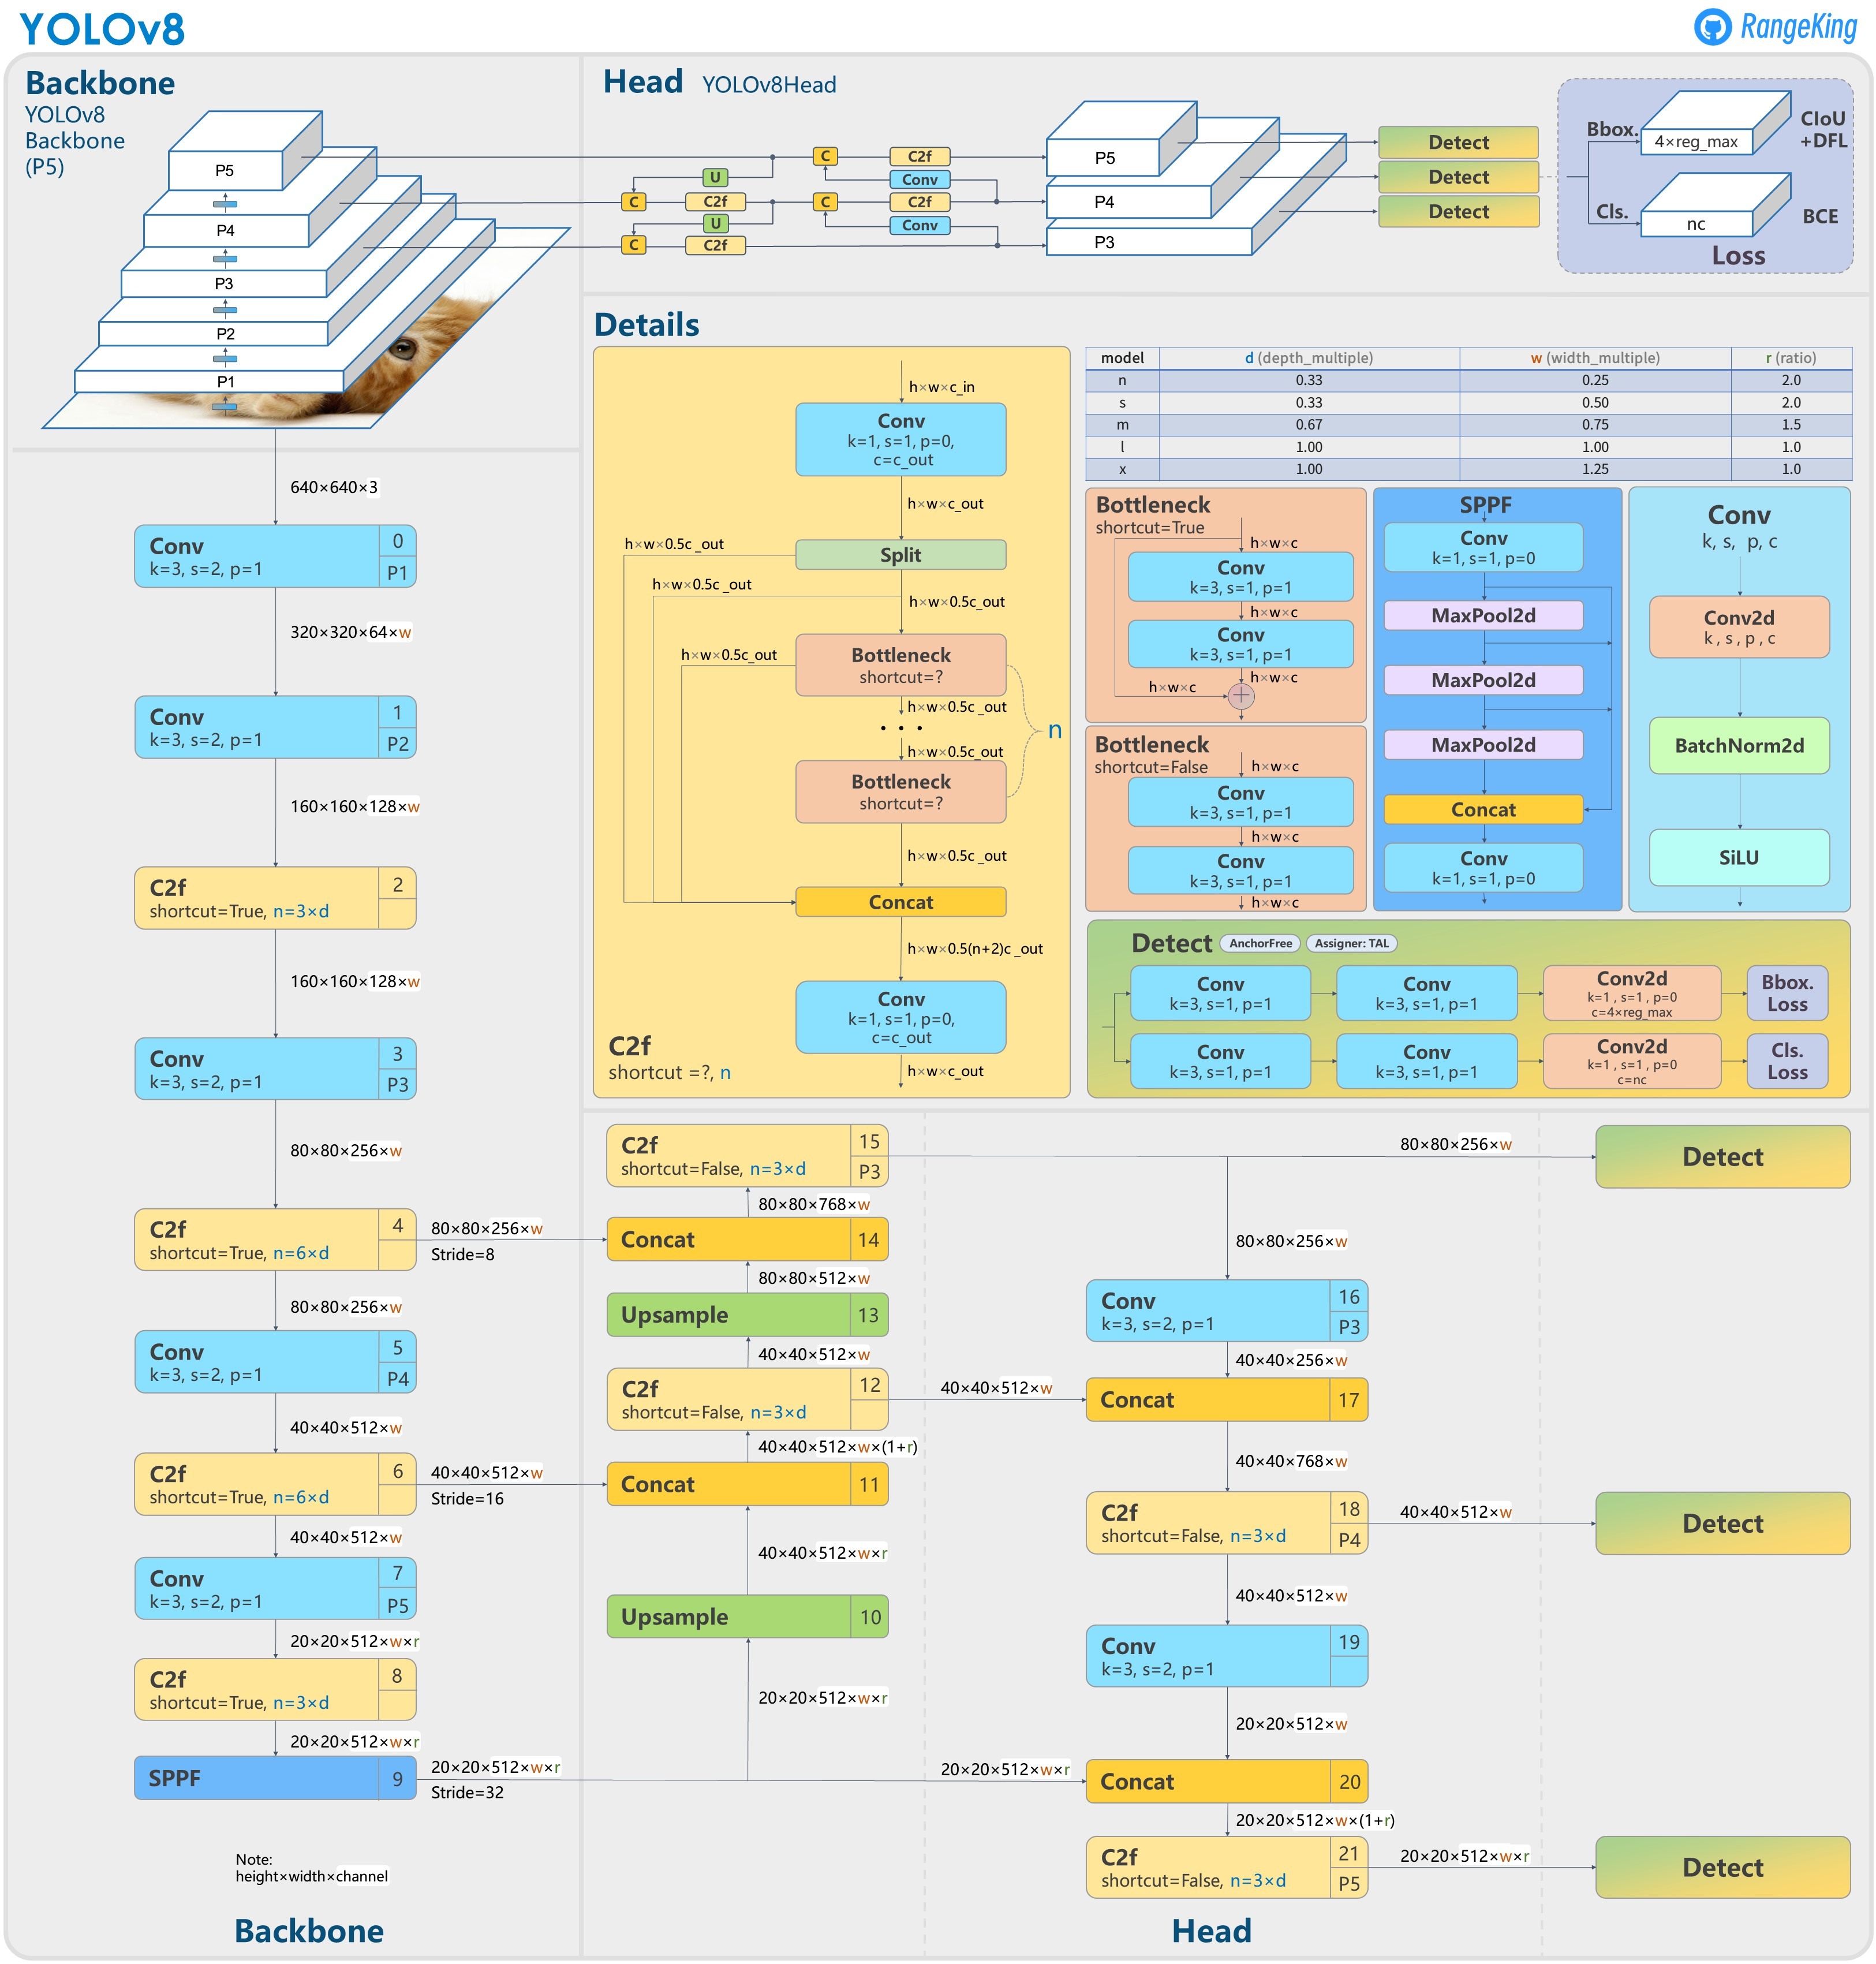
\includegraphics[width=0.8\linewidth]{images/yolov8.jpg}
    \caption{\label{fig:yolov8_issue189} Figura que ilustra a arquitetura do YOLOv8. Imagem extraída de \citeauthor{ultralytics_issue_189}. Disponível em: \url{https://github.com/ultralytics/ultralytics/issues/189}.}
\end{figure}

Essas inovações resultaram em um desempenho superior do \emph{YOLOv8} em comparação com suas versões anteriores. Em testes realizados no conjunto de dados COCO, o \emph{YOLOv8} demonstrou um aumento no \emph{Mean Average Precision} (mAP) e uma velocidade de inferência mais rápida \citep{ultralytics_yolov8_results}.

Infelizmente, não houve a publicação de um artigo científico oficial da \emph{Ultralytics} para que possamos saber com facilidade o passo a passo do funcionamento do modelo \emph{YOLOv8}. Além disso, o repositório do \emph{Github} que contém a codificação da arquitetura do modelo está passando por atualizações constantes, com as modificações do código fonte do \emph{YOLOv8} para novos códigos, que originaram o \emph{YOLO11}. Dessa forma, consideramos que a profundidade da explicação feita sobre o \emph{YOLOv8} é o bastante para o intuito desse trabalho de formatura supervisionado.


\section{Materiais e métodos}
\label{sec:treinamento}
Depois de escolhermos o modelo \emph{YOLOv8} para realizar a detecção de objetos no projeto \emph{TomatoHealth}, chegou o momento de treiná-lo para que ele tivesse a capacidade de detectar as doenças em folhas de tomate. Como comentado anteriormente, o \emph{dataset} escolhido para essa tarefa foi o \emph{PlantDoc}, mas com o escopo reduzido para doenças em folhas de tomate.

\subsection{Processamento do \emph{dataset}}
Para obtermos o \emph{dataset} das doenças em folhas de tomate, precisamos então realizar uma filtragem no \emph{PlantDoc} para que somente imagens que possuam rótulos de doenças de tomate (e esses rótulos em si) permanecessem na versão do \emph{dataset} que seria utilizada para treinar o modelo.

Para fazer isso, primeiro obtemos o conjunto de dados \emph{PlantDoc} a partir da plataforma \emph{Dataset Ninja}\footnote{\url{https://datasetninja.com/plantdoc}} --- essa plataforma disponibiliza conjuntos de dados para uso em projetos de \emph{Machine Learning}. Depois disso, no processo de filtragem do \emph{dataset}, também precisamos fazer adaptações no formato dos \emph{rótulos} e da estrutura de diretórios para que tivéssemos um conjunto de dados adaptado para a arquitetura \emph{YOLO}.

Sobre os rótulos, o formato inicial define as \emph{bounding boxes} a partir do seu vértice superior esquerdo e do seu vértice inferior direito. Então precisamos fazer uma transformação para obter o tamanho, largura e centro de cada caixa. O código responsável por esse processamento pode ser encontrado no repositório de códigos do projeto\footnote{\url{https://github.com/heitorc62/TCC}}.

Inicialmente, a estrutura de diretórios apresentava o seguinte formato:
\begin{verbatim}
treino/
|-- imgs/
|-- rótulos/
teste/
|-- imgs/
|-- rótulos/
\end{verbatim}
Para o uso com o \emph{YOLO}, a organização de diretórios precisa ser ajustada para separar as imagens e os rótulos em diretórios específicos, com subdiretórios para treino e teste. A estrutura correta é:
\begin{verbatim}
imgs/
|-- treino/
|-- teste/
rótulos/
|-- treino/
|-- teste/
\end{verbatim}
Ao final de todo esse processamento, restaram as seguintes classes no \emph{dataset}:

\begin{table}[h!]
\centering
\resizebox{\textwidth}{!}{
\begin{tabular}{|c|l|l|}
\hline
\textbf{ID} & \textbf{Nome Original (Inglês)} & \textbf{Nome em Português} \\
\hline
0 & Tomato Early blight leaf & Folha de tomate com pinta-preta \\
1 & Tomato leaf & Folha de tomate saudável \\
2 & Tomato leaf bacterial spot & Folha de tomate com mancha bacteriana \\
3 & Tomato leaf late blight & Folha de tomate com requeima \\
4 & Tomato leaf mosaic virus & Folha de tomate com vírus do mosaico \\
5 & Tomato leaf yellow virus & Folha de tomate com Begomovirus (yellow leaf curl virus) \\
6 & Tomato mold leaf & Folha de tomate com mofo \\
7 & Tomato Septoria leaf spot & Folha de tomate com septoriose (fungo) \\
8 & Tomato two spotted spider mites leaf & Folha de tomate com ácaro-rajado (spider mite) \\
\hline
\end{tabular}
}
\caption{Nomes originais das classes e suas traduções em português.}
\label{tab:class-names}
\end{table}

\begin{figure}[htb!]
    \centering
    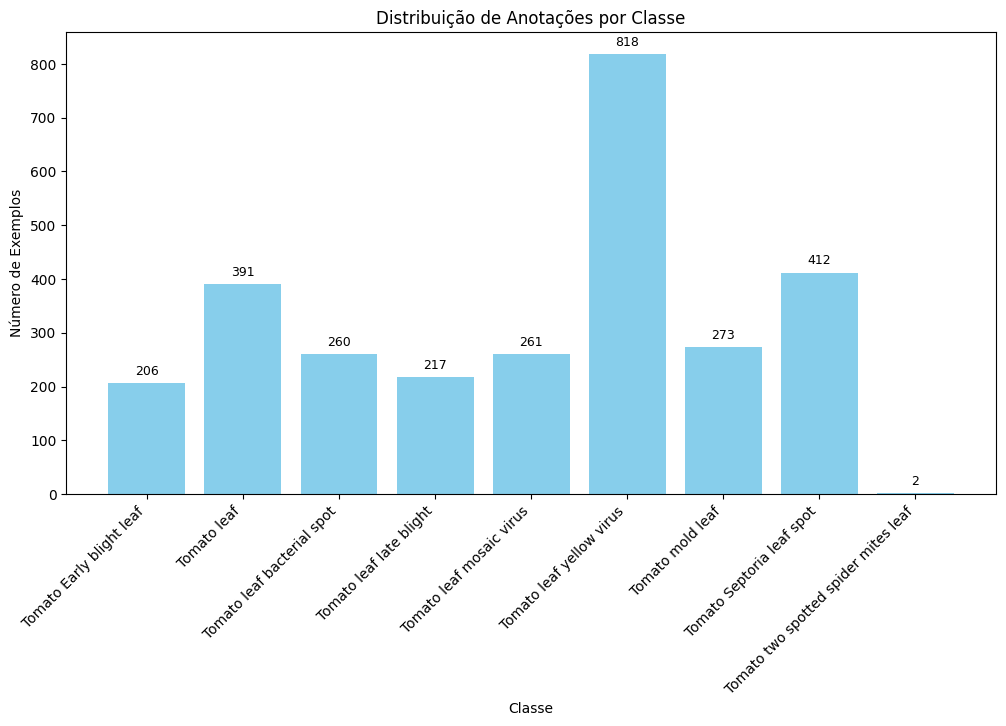
\includegraphics[width=1\linewidth]{images/distribuicao_anotacoes.png}
    \caption{\label{fig:distribuicao-ann-cls} Gráfico de barras mostrando a distribuição de anotações por classe após o processamento do conjunto de dados PlantDoc. Fonte: acervo dos autores.}
\end{figure}

Totalizando 721 imagens, 2840 anotações e uma média de 3.93897 anotações por imagem. Na figura \ref{fig:distribuicao-ann-cls} é possível enxergar a distribuição de anotações por classes. É notável que a classe \emph{Tomato two spotted spider mites leaf} possui um número muito pequeno de exemplos. Contudo, como o intuito do projeto é, justamente estender o atual conjunto de dados com novas imagens e novas anotações, decidimos não desconsiderar essa classe e mantê-la no conjunto de dados.

\subsection{Treinamento}
\label{sec:treinamento2}
Após o pré-processamento, o conjunto de dados foi adequadamente estruturado para ser utilizado pelo \emph{YOLO}. Com isso, o próximo passo foi realizar o treinamento do modelo. Executamos um processo de ajuste fino (\emph{fine-tuning}) do \emph{YOLOv8n} (uma versão mais leve do \emph{YOLOv8}), previamente treinado no \emph{dataset} COCO\footnote{\url{https://yolov8.org/yolov8-coco-dataset/}} \cite{COCO}.

Para realizar o ajuste fino, foram utilizadas duas abordagens principais:

\begin{itemize}
    \item \textbf{Linha de comando com \emph{Bash}}: A primeira opção é rodar o treinamento diretamente no terminal com um comando \emph{bash}, que especifica configurações, como a tarefa, o número de épocas e o tamanho da imagem:

\begin{lstlisting}
    yolo task=detect mode=train model=yolov8n.pt data=tomato.yaml epochs=300 imgsz=640 device=0 
\end{lstlisting}

   \begin{itemize}
       \item \texttt{task=detect}: define a tarefa como detecção de objetos.
       \item \texttt{model=yolov8n.pt}: indica o modelo \emph{YOLOv8} pré-treinado a ser utilizado.
       \item \texttt{data=tomato.yaml}: aponta para o arquivo de configuração dos dados, que mapeia as classes para seus nomes e os caminhos das imagens.
       \item \texttt{epochs=50}: número de épocas para o treinamento.
       \item \texttt{imgsz=640}: define o tamanho das imagens usadas no treinamento.
       \item \texttt{device=0}: especifica o dispositivo (\emph{GPU}) para acelerar o treinamento.
   \end{itemize}

    \item \textbf{Uso da biblioteca \emph{Python} da \emph{Ultralytics}}: A segunda opção é utilizar funções disponibilizadas pela biblioteca de \emph{Python} da \emph{Ultralytics}:
    \begin{lstlisting}
       results = model.train(task="detect", data=data_yaml, epochs=epochs, imgsz=img_size, device=device)
    \end{lstlisting}
\end{itemize}
Para treinar o modelo, utilizamos a rede de computadores (\emph{vision, e-science}) com placas de vídeo (\emph{GPU}). Mais especificamente a máquina chamada \emph{deepthree}, com 200\emph{GB} de RAM e equipada com a placa de vídeo \emph{NVIDIA GeForce GTX 1080 Ti} com 12\emph{GB} de memória.

\subsection{Resultados}
\label{sec:resultados}
Com o \emph{dataset} que obtivemos após o processamento e utilizando o \emph{YOLOv8n}, decidimos fazer um treinamento por 300 épocas. As ferramentas fornecidas pela \emph{Ultralytics} facilitam muito esse processo. O parâmetro \emph{EarlyStopping(patience=100)} define que o treinamento para após 100 épocas sem melhorias nas métricas de avaliação. Então, após 183 épocas o treinamento foi finalizado já que o melhor modelo encontrado foi do final da época de número 83. O treino com 183 épocas e utilizando as configurações de hardware mencionadas na seção \ref{sec:treinamento2}, leva cerca de 30 minutos e resulta em um arquivo de pesos de cerca de 6\emph{MB}. Os resultados obtidos podem ser vistos na figura \ref{fig:resultados-treinamento}.

\begin{figure}[htb!]
    \centering
    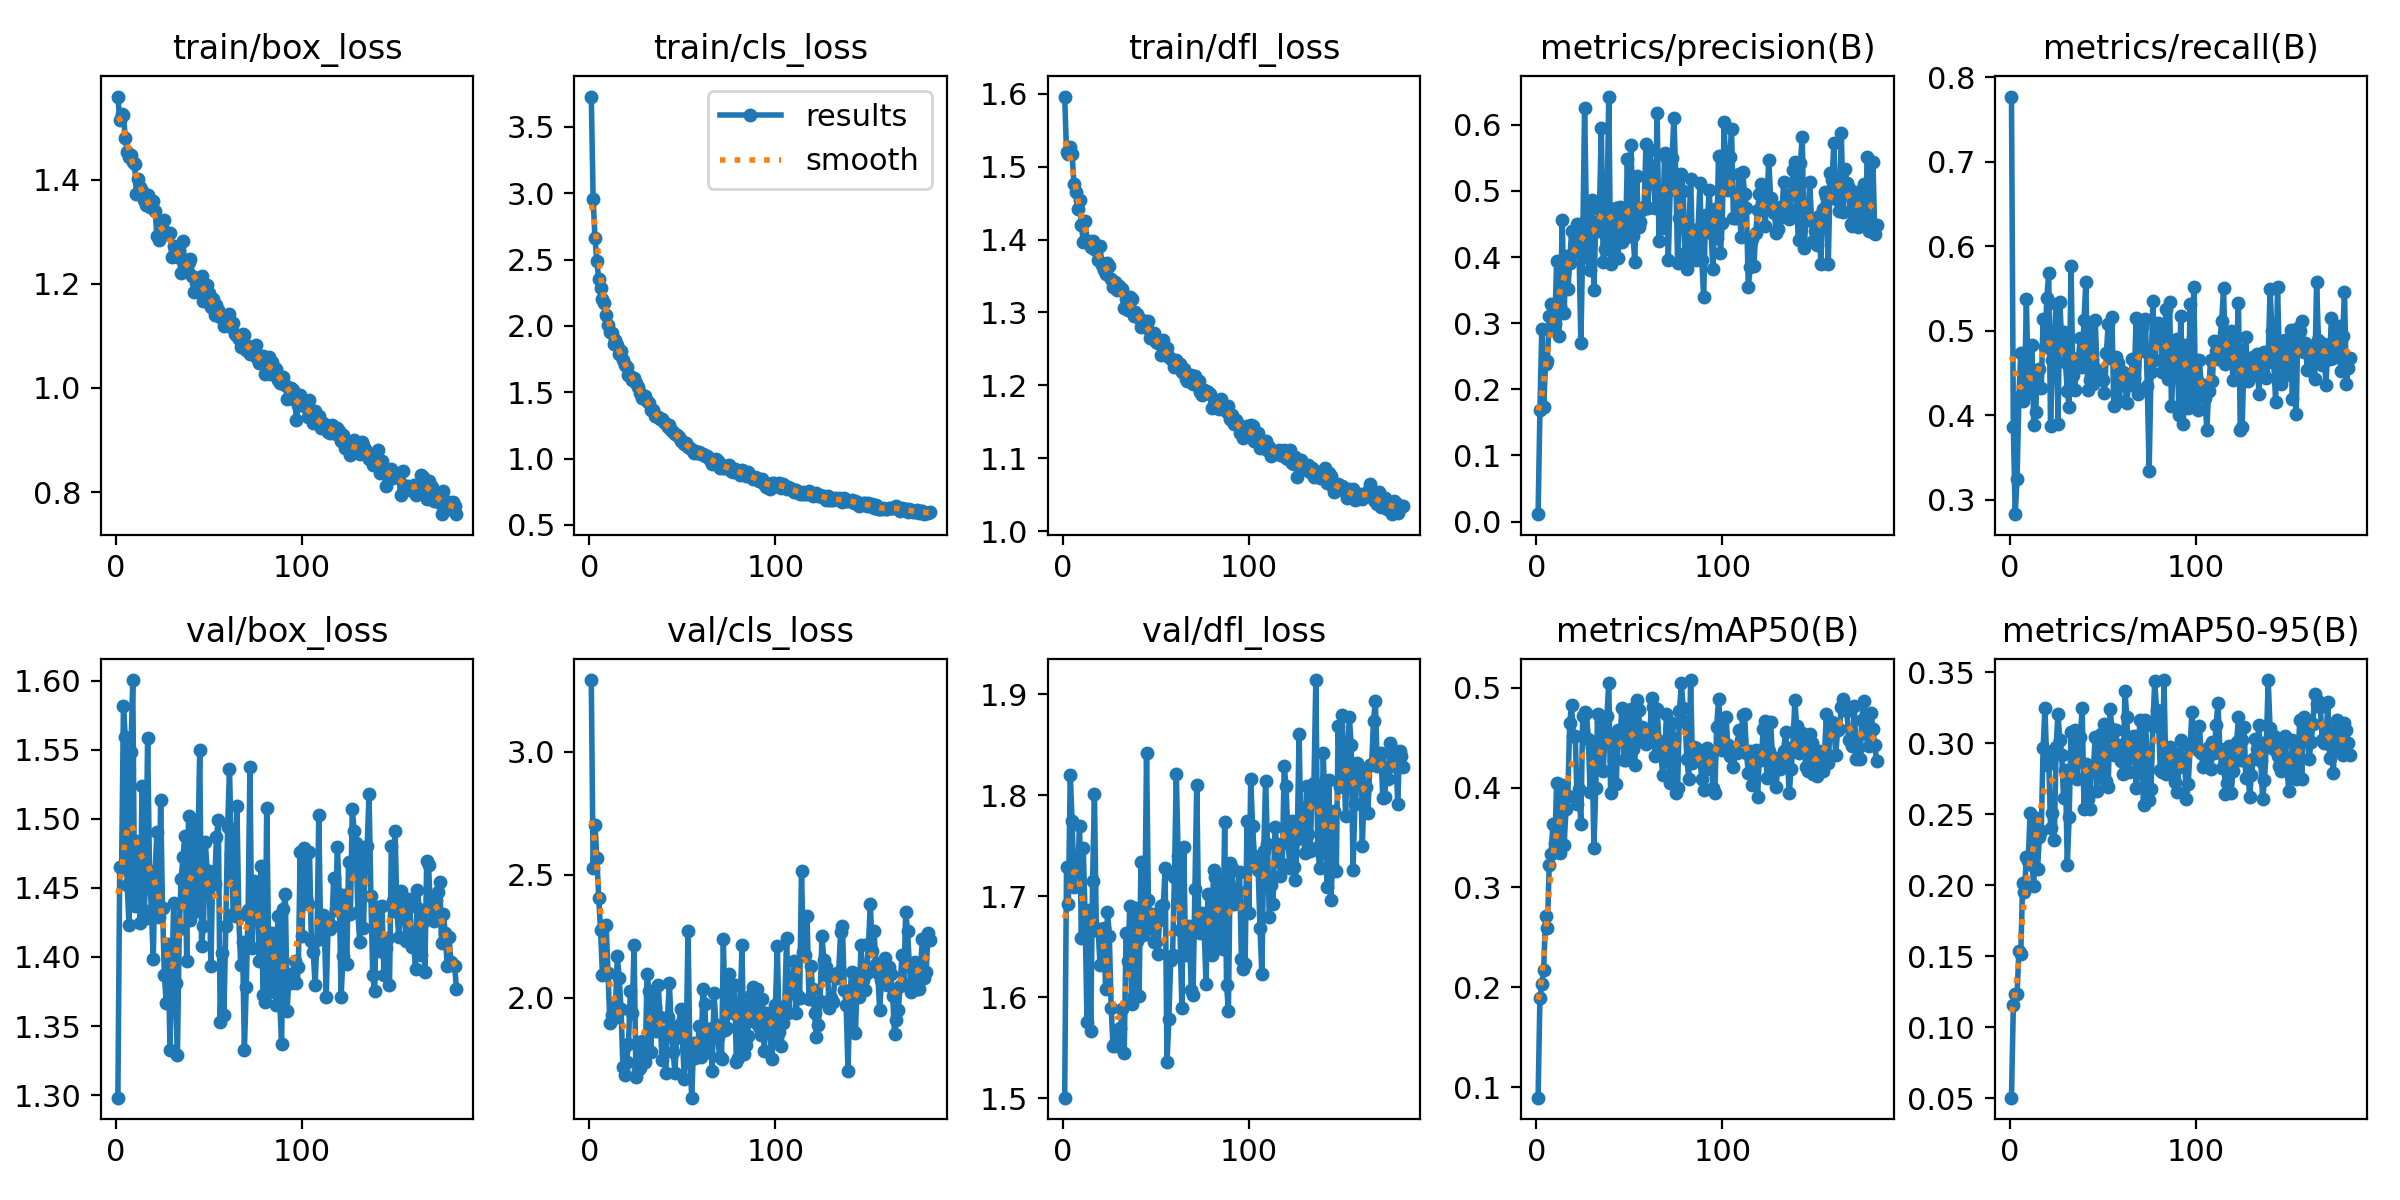
\includegraphics[width=1\linewidth]{images/results.png}
    \caption{Resultados obtidos após 183 épocas de treinamento. Fonte: acervo dos autores.}
    \label{fig:resultados-treinamento}
\end{figure}

O melhor valor da métrica \emph{mAP\string@50-95} obtido após o treinamento foi: 34,437; Se compararmos esse valor com os melhores resultados do \emph{YOLOv8} na referência de performance do \emph{dataset COCO} (37.3) conseguimos notar que, pelo menos na teoria, o conjunto de dados está performando bem.

Apesar do intuito do \emph{TomatoHealth} ser a construção de um conjunto de dados robusto no domínio de detecção de doenças em folhas de tomate, pensamos que em um momento inicial é interessante ter um modelo que seja o melhor possível. 

Assim, devido ao pequeno número de exemplos que possuímos inicialmente nesse \emph{dataset}, reconhecemos que essa métrica de 34,437 pode estar superestimada e isso pode ser observado nas figuras \ref{fig:val-pred} e \ref{fig:val-labels} (predições incorretas no conjunto de validação). Então, consideramos uma estratégia para tentar melhorar essa performance inicial. Essa estratégia será discutida na seção \ref{sec:integrando-resultados}.
\begin{figure}[H]
    \centering
    \begin{subfigure}[t]{0.45\textwidth}
        \centering
        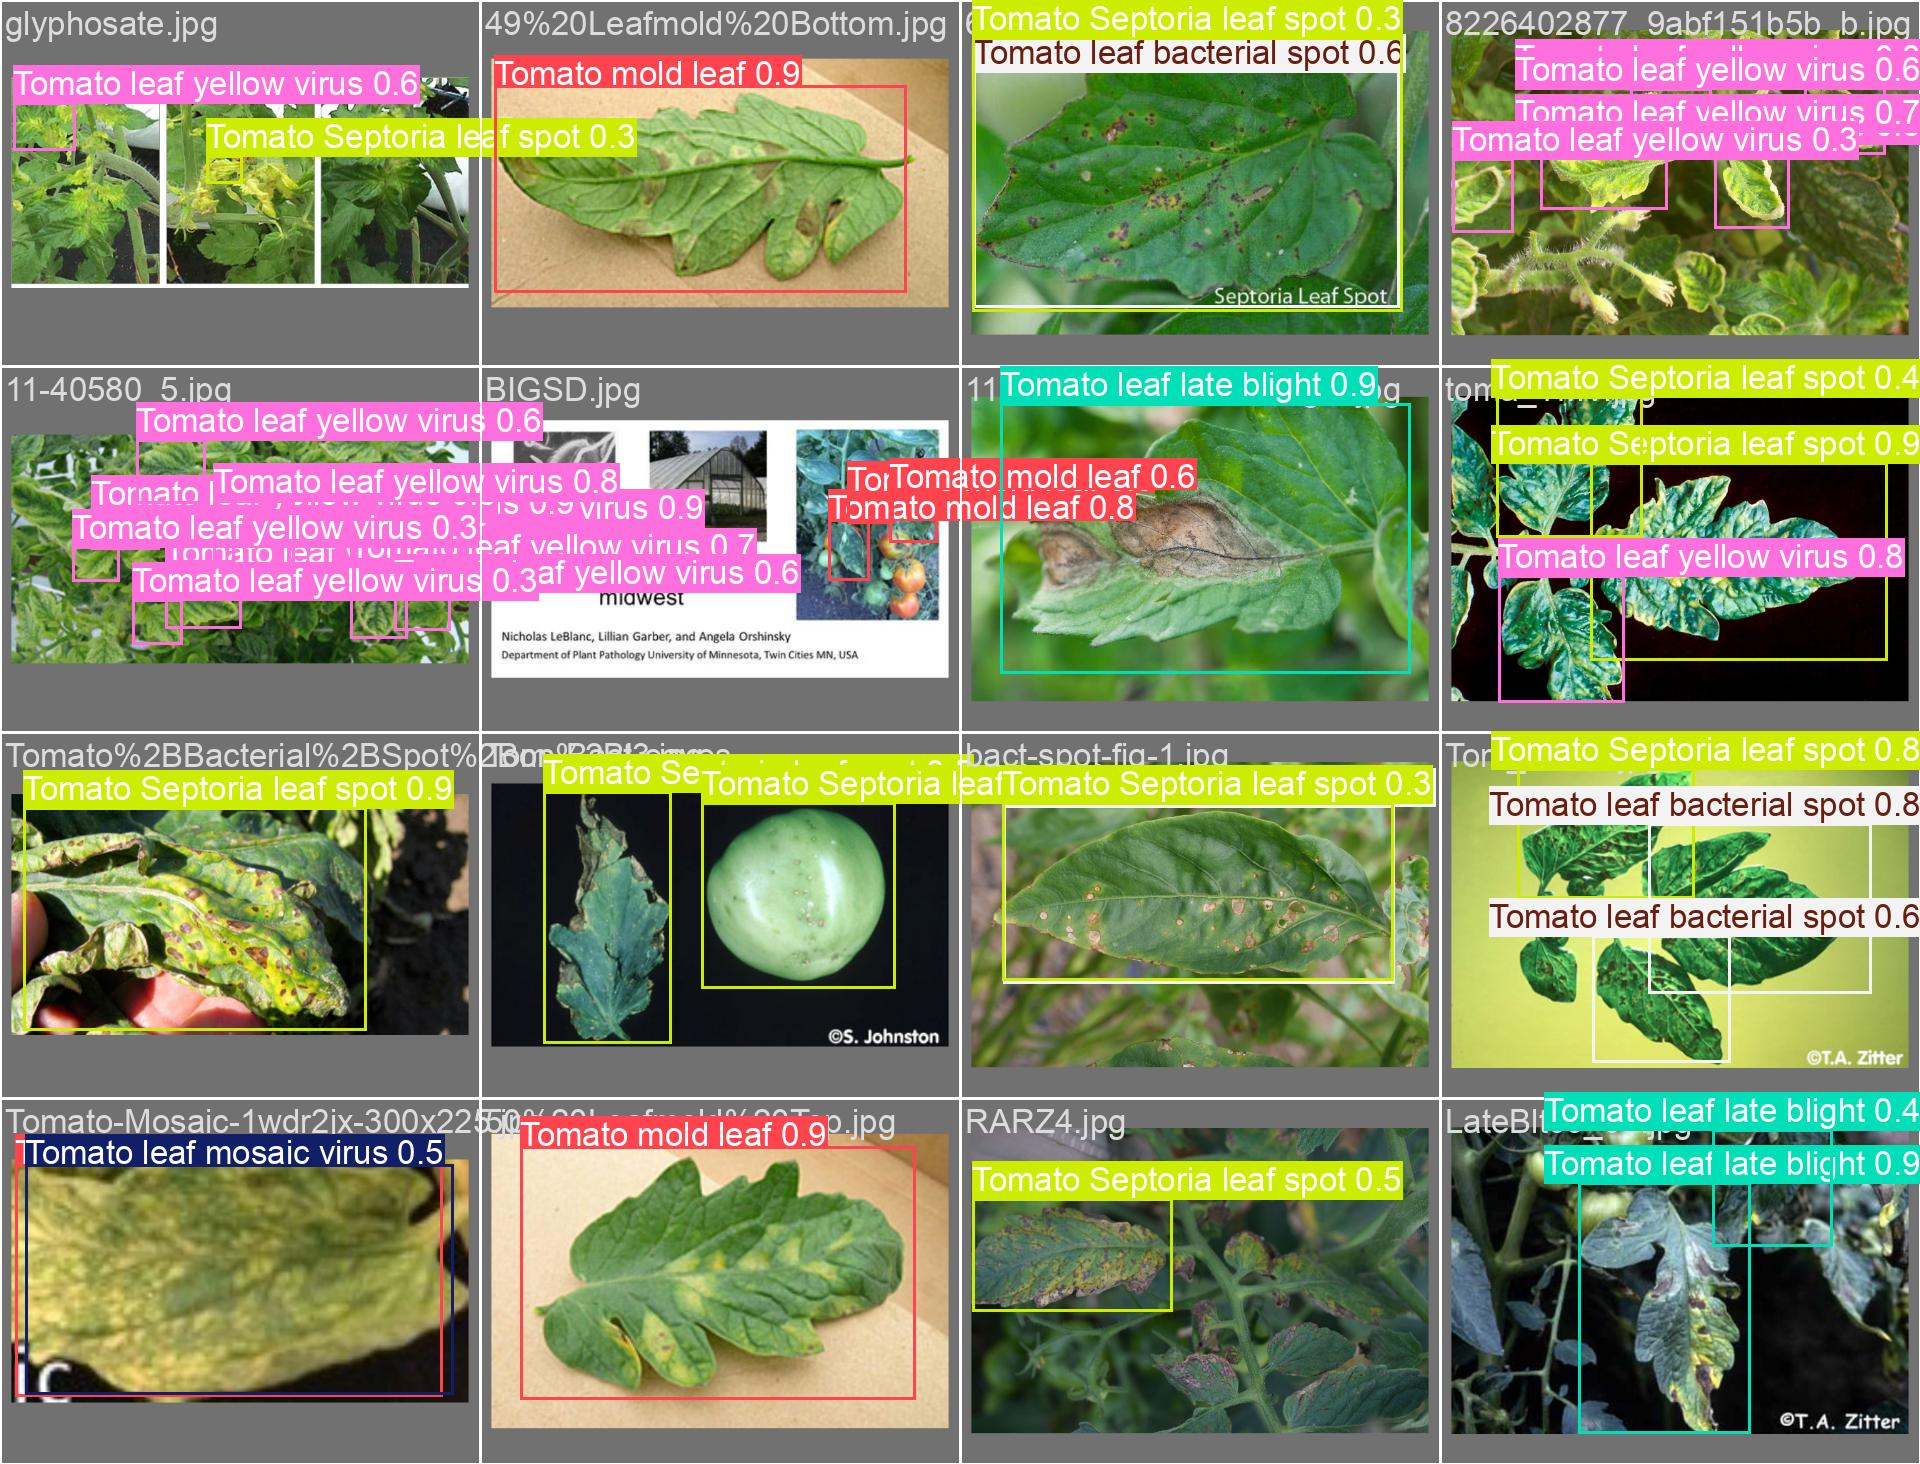
\includegraphics[width=\textwidth]{images/val_batch0_pred.jpg}
        \caption{Exemplo de deteccao de objetos em imagens do conjunto de validação. Imagem extraída do acervo dos autores.}
        \label{fig:val-pred} 
    \end{subfigure}\hfill
    \begin{subfigure}[t]{0.45\textwidth}
        \centering
        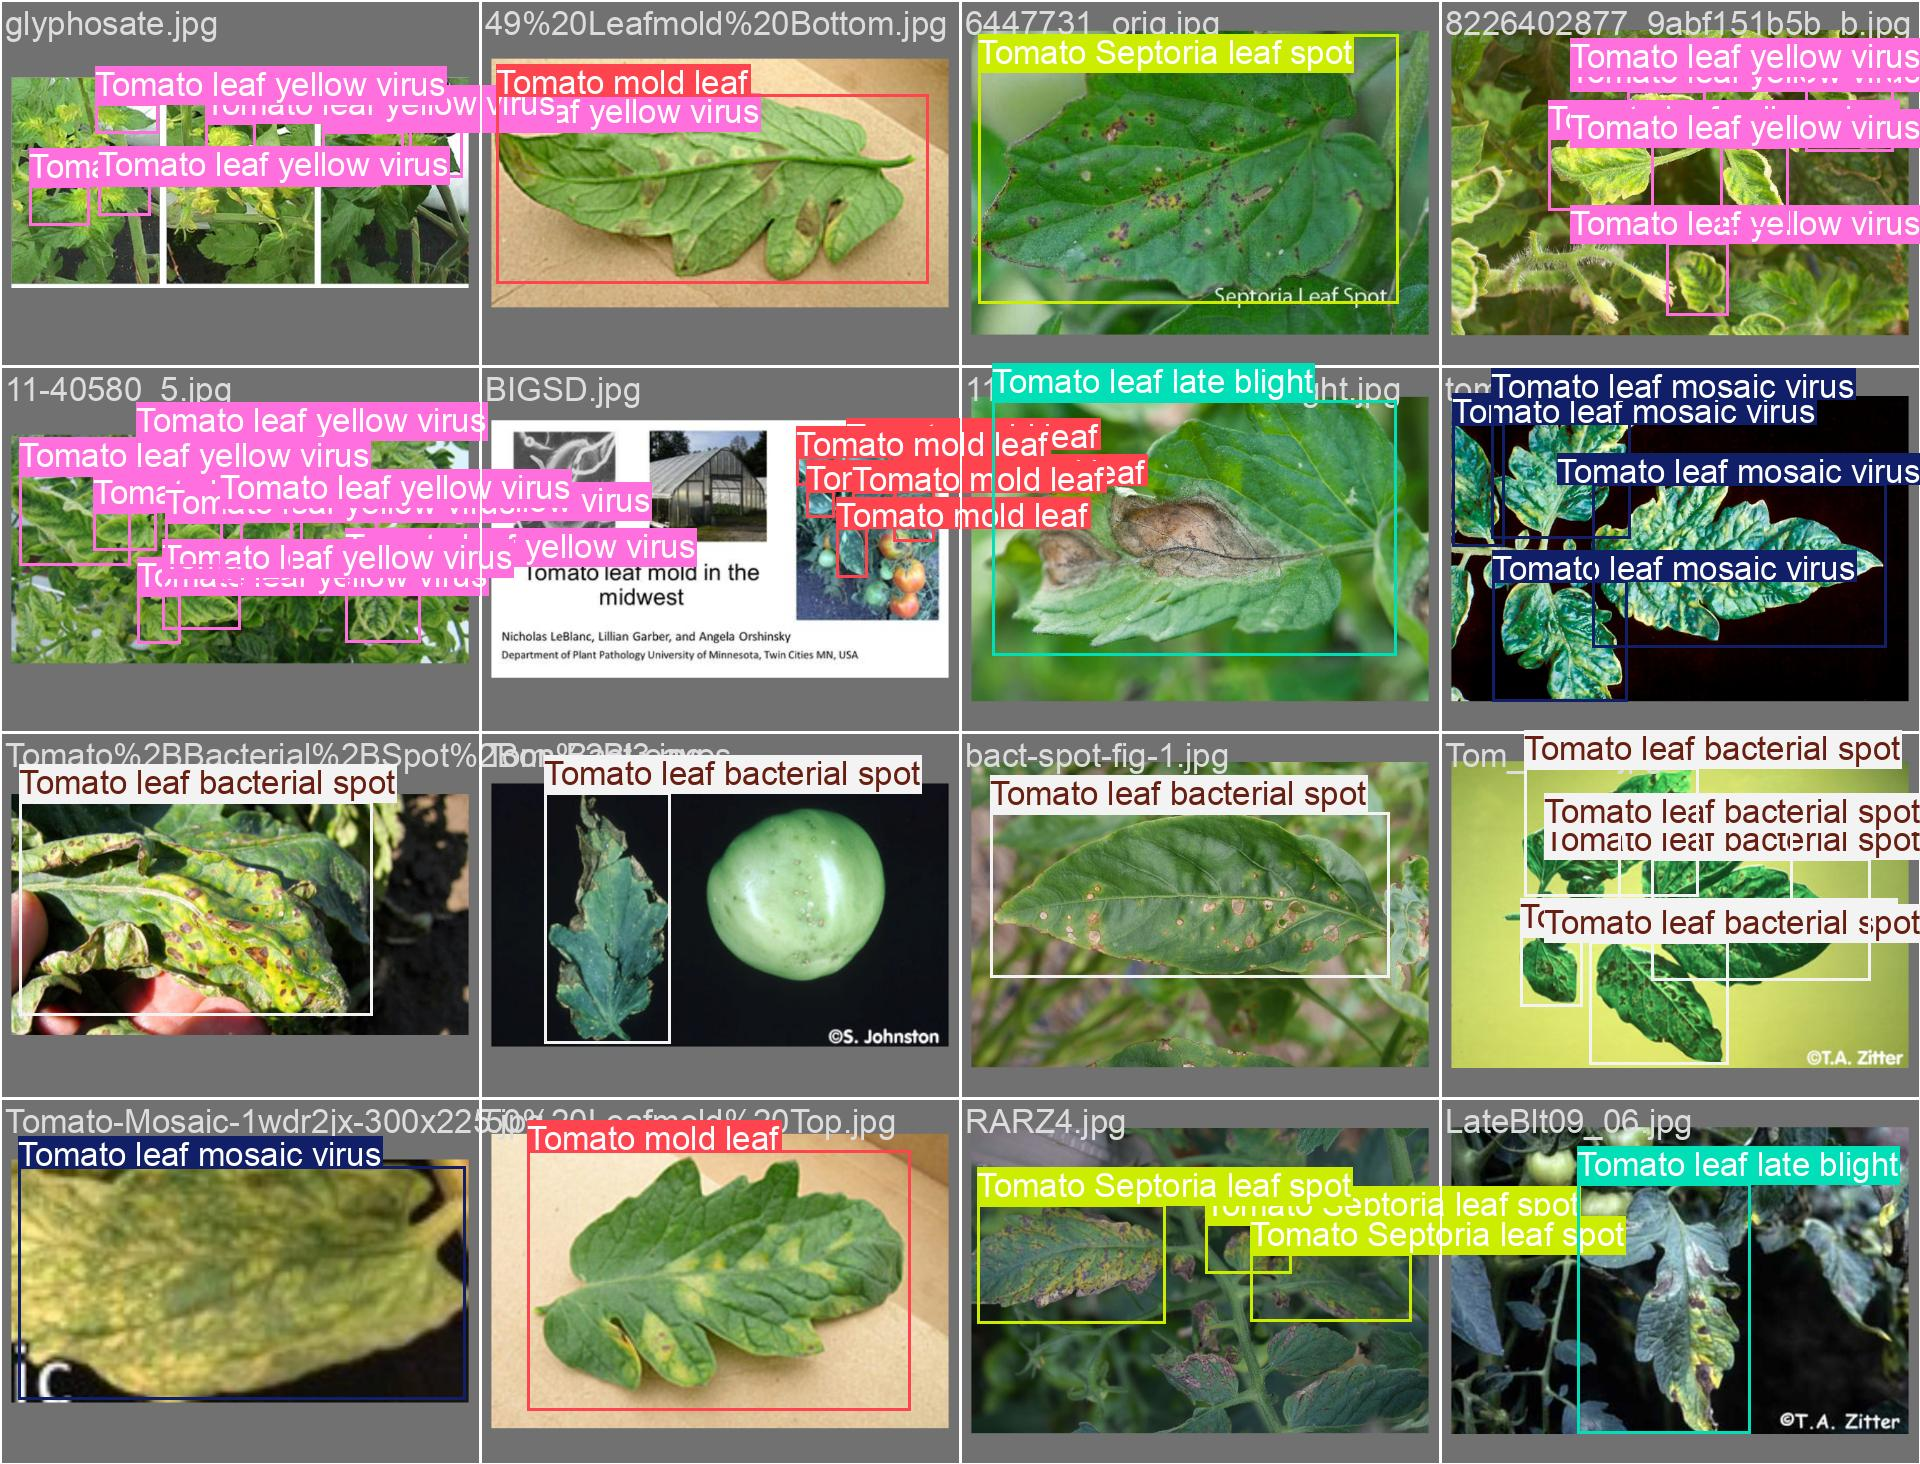
\includegraphics[width=\textwidth]{images/val_batch0_labels.jpg}
        \caption{Exemplo de rotulos de objetos. Imagem extraída do acervo dos autores.}
        \label{fig:val-labels}
    \end{subfigure}
    \caption{Comparação entre a detecção de objetos e os rotulos originais.}
    \label{fig:comparison}
\end{figure}